\documentclass[11pt]{article}
\usepackage[a4paper,margin=2.5cm]{geometry}
\usepackage{fontspec}
\setmainfont{Noto Sans KR}[BoldFont={Noto Sans KR}, BoldFeatures={FakeBold=2.2},
  ItalicFont={Noto Sans KR}, ItalicFeatures={FakeSlant=0.18}]
\usepackage{amsmath,amssymb}
\usepackage{graphicx}
\usepackage{booktabs}
\usepackage{xcolor}
\usepackage{hyperref}
\usepackage{tikz}
\usetikzlibrary{arrows.meta,positioning,calc,shapes.geometric,fit,backgrounds,decorations.pathreplacing}
\usepackage{caption}
\usepackage{kotex}
\hypersetup{colorlinks=true, linkcolor=blue!50!black, citecolor=blue!50!black, urlcolor=blue!40!black}
\setlength{\emergencystretch}{3em}
\newcommand{\pending}[1]{\textcolor{red!70!black}{\textbf{[결과 대기: #1]}}}

\usepackage{tabularx}
\usepackage{longtable}
\usepackage{multirow}
\usepackage{enumitem}
\usepackage{fancyvrb}
\usepackage[section]{placeins}
\setmonohangulfont{Noto Sans KR}[BoldFont={Noto Sans KR}, BoldFeatures={FakeBold=2.2}]
\setlist{itemsep=2pt, topsep=4pt}
\captionsetup{font=small, labelfont=bf}
% config key: printed as typed, with a line-break allowed after every underscore
\ExplSyntaxOn
\tl_new:N \l__key_tl
\DeclareRobustCommand{\key}[1]{
  \tl_set:Nx \l__key_tl { \tl_to_str:n {#1} }
  \regex_replace_all:nnN { \_ } { \cO\_ \c{allowbreak} } \l__key_tl
  \texttt{ \tl_use:N \l__key_tl }
}
\ExplSyntaxOff
\newcommand{\wide}[2]{\makebox[\textwidth][c]{\includegraphics[width=#1]{#2}}}
\newcolumntype{L}{>{\raggedright\arraybackslash}X}
\definecolor{tealx}{HTML}{1f7a78}
\definecolor{redx}{HTML}{c0392b}
\AtBeginDocument{\renewcommand{\contentsname}{차례}\renewcommand{\figurename}{그림}\renewcommand{\tablename}{표}}

\title{\textbf{SDFFlow 형상 생성 모델}\\[4pt]\large 쉽게 풀어 쓴 설명서: 구조, config 작성법, ex3 너트 실험, DeepJEB 진행 상황}
\author{AI-CAE4ALL}
\date{2026년 9월 28일 기준 (대표점 수 연구 추가)}

\begin{document}
\maketitle

\noindent 이 문서는 \texttt{methods/SDFFlow}가 무엇을 하는지, config를 어떻게 써야 하는지,
지금까지 실험에서 무엇을 알았는지를 한곳에 정리한 것이다. 어려운 전산 용어 대신 풀어 쓴 말을 쓰고,
config에 적는 이름(key)만 \key{이런_글꼴}로 적는다. 풀어 쓴 말과 흔히 쓰는 용어의 대조표는
부록~\ref{app:glossary}에 있다. 아직 끝나지 않은 실험의 결과 자리는 \pending{설명}처럼 빨간 글씨로 표시했다.

\section*{한눈에 보기: 질문별 짧은 답}
\addcontentsline{toc}{section}{한눈에 보기}

\begin{description}[leftmargin=0pt, style=nextline, itemsep=5pt]
\item[``VAE 입력이 32토큰? 32채널이 뭐야?'']
입력은 토큰이 아니라 형상 표면에서 뽑은 점 6144개(좌표와 면 방향)이다. 모델은 이 가운데 서로 멀리
떨어진 점 $T$개를 \textbf{대표점}으로 고르고, 각 대표점이 표면 점 전체를 훑어 자기 주변 모양을 숫자
32개로 요약한다. 그래서 형상 하나는 ``대표점 $T$개 $\times$ 숫자 32개''의 표(\textbf{형상 코드})가 된다.
ex3는 $T=32$라 $32\times32=1024$개, DeepJEB 실험 J0--J2는 $T=512$라 $512\times32=16384$개 숫자다
(\S\ref{sec:vae}, 그림~\ref{fig:grid}).
\item[``출력은 임의의 점에서 SDF 값이지?'']
그렇다. 복원부(형상 코드를 받아 형상으로 되돌리는 부분)는 공간의 아무 점이나 받아서 그 점의 부호 거리(안쪽은 음수, 바깥은 양수, 표면은 0)를
하나 돌려준다. 학습할 때는 $\pm0.1$보다 먼 값은 잘라낸다. STL을 만들 때는 $128^3$ 격자 점마다 이 값을
계산하고 값이 0인 면을 뽑는다(\S\ref{sec:sdf}, \S\ref{sec:mesh}).
\item[``그럼 $(T, 256)$ $\rightarrow$ 요약부 $\rightarrow$ 형상 코드 $\rightarrow$ 복원부 $\rightarrow$ $(T, 1)$인가?'']
아니다. 두 군데가 다르다. 첫째, 요약부의 입력은 $(T, 256)$이 아니라 표면 점 $(6144, 6)$이다. $(T, 256)$은 요약부
\emph{안에서} 대표점 $T$개의 줄만 골라 온 중간 값이다. 둘째, 복원부의 출력은 $(T, 1)$이 아니라 $(M, 1)$이다.
$M$은 부호 거리를 물어본 질문 점의 개수로, 학습할 때 8192개, STL을 만들 때 $128^3$개다. 대표점 $T$개는
답을 내는 자리가 아니라, 질문 점마다 훑어보는 참고 줄이다(\S\ref{sec:vaeshapes}, 그림~\ref{fig:vaeshapes}).
\item[``대표점 $T$와 표면 점 수는 무조건 클수록 좋은 것 아닌가?'']
복원만 보면 대표점이 많을수록 좋다. DeepJEB에서 $T=512$(J1)의 점검용 복원 오차는 $T=32$(J3)의 약 2.6분의 1이다.
그러나 형상 코드의 숫자가 16배(1024개 $\rightarrow$ 16384개)로 늘어서, 같은 벌점 가중치에서 벌점이 16배 세지고
(J0는 이 때문에 무너졌다), 2단계가 만들어야 할 숫자도 16배가 된다. 실제로 2단계까지 같은 500바퀴로 학습하니
\textbf{생성은 오히려 나빠졌다}. 조건 없이 만든 형상 중 한 조각인 비율이 72\%(J3)에서 31\%(J1)로, 실제 조건을 주었을 때의
부피 오차가 2.5\%에서 8.3\%로 나빠졌다(\S\ref{sec:jebeval}). 2단계를 네 배 오래 학습해도 거의 그대로였다(38\%).
형상마다 코드를 여러 개 뽑아 2단계 자료를 늘리고, 학습 시점을 잡음 쪽으로 치우치고, 2단계를 키우면 512도 32 수준까지 오르지만
넘지는 못했고 2단계 시간이 약 20배다. MCB와 DrivAerML에서도 같았다. 대표점 128에 같은 처방을 하면 복원은 1.7배 좋고 생성은 32와 같아
균형이 가장 좋았다(\S\ref{sec:tsize}). 학습 형상이 수천 개 이하인 지금은 32가 작지 않다. 표면 점 수는 저장된 8192개가 상한이고, 6144개를 매번 새로 뽑는 것 자체에도 쓸모가 있다(\S\ref{sec:vaeshapes}).
\item[``Flow matching은 임의의 잡음에서 조건에 맞게 VAE 코드를 예측하는 것?'']
거의 맞다. 정확히는 한 번에 ``예측''하지 않고 \textbf{50걸음에 걸쳐 조금씩 옮긴다}. 생성 모델은
``지금 위치, 진행 정도, 조건''을 받아 ``어느 쪽으로 가야 하는지''를 알려 주고, 잡음에서 출발해 그 방향으로
50번 걸으면 형상 코드에 도착한다. 걸음은 매번 똑같이 계산되므로 같은 잡음과 같은 조건이면 항상 같은 형상이
나온다(\S\ref{sec:fm}).
\item[``결과는 어쨌든 kl 1e-8부턴 좋은 거네?'']
ex3에서는 \textbf{1e-6부터} 이미 좋다. 기준은 가중치 숫자 자체가 아니라
``가중치 $\times$ 형상 코드의 숫자 개수''이며, 이 값이 약 $10^{-3}$ 이하이면 정상이었다. 같은 1e-6도
숫자가 1024개인 ex3에서는 정상이고, 16384개인 DeepJEB J0에서는 코드가 무너졌다(\S\ref{sec:kl}).
\item[``kl 1e-6이어도 castle 점검용 결과가 안 좋다. 압축 모델 자체가 부족한 것 같다'']
맞다. 다만 부족한 곳이 정해져 있다. 점검용과 학습용의 오차 \emph{중앙값}은 같지만,
점검용/학습용 오차 비율이 육각 너트는 1.05배, 잠금 너트는 2.4배, 캐슬 너트는 10배다.
캐슬 너트는 정답 형상을 같은 격자로 뽑아도 한 조각으로 나오는 비율이 66.7\%뿐이다(\S\ref{sec:castle}).
\item[``1단계, 2단계 학습 바퀴 수가 충분한가?'']
1단계(압축 모델)는 충분하다. 약 500바퀴부터 점검용 오차가 평탄하고, 가장 좋은 지점은 625--885바퀴였다.
2단계(생성 모델)는 500바퀴면 조금 모자라다. 약 700바퀴로 늘리고 가장 좋았던 시점의 파일
(\key{fm_best.pth})을 쓰는 것을 권한다(\S\ref{sec:epochs}).
\item[``보간(interpolation) STL 상태가 그래도 안 좋다'']
맞다. 가중치를 낮추면 떨어진 조각은 거의 사라진다. 남은 문제는 경로다. 섞는 도중에 구멍이 닫혔다가
끝에서 갑자기 다시 뚫리고, 세워진 너트가 한순간에 눕혀진 너트로 바뀐다. 이 ``튐''의 상당 부분은 ex3 데이터에
같은 너트가 세워지거나 눕혀진 채로 섞여 있기 때문이었다(\S\ref{sec:orient}).
\item[``조건부로 해 봐야 하나?'']
도움은 되지만 핵심은 아니다. 실제 두 형상 사이를 조건까지 함께 옮기면 경로가 더 고르게 변한다.
하지만 구멍이 닫혔다 열리는 현상과 캐슬 너트 조각은 그대로다. 조건을 하나로 고정하면 튐이 없어지는데,
그것은 형상이 거의 움직이지 않기 때문이다(\S\ref{sec:cond}).
\item[``DeepJEB에 대해서 돌릴 거지?'']
돌렸다. aarl GPU 0--2에서 J1, J2, J3 세 실험이 두 단계를 모두 마쳤고(9월 26일 J3 06:36, J1 15:53, J2 16:14),
생성·섞기 평가도 J0를 포함한 네 모델에 똑같이 돌렸다(16:37 끝). 세 실험 모두 1단계가 무너지지 않았고,
생성과 섞기는 대표점 32개인 J3가 가장 좋았다(\S\ref{sec:jeb}, \S\ref{sec:jebeval}).
같은 부모의 형제끼리와 다른 부모끼리를 나눈 보간 평가는 아직 하지 않았다.
대표점 수는 9월 26--28일에 따로 다시 확인했다(\S\ref{sec:tsize}).
\end{description}

\tableofcontents
\clearpage

% ======================================================================
\section{큰 그림: 두 단계로 나뉜 모델}
\label{sec:overview}

SDFFlow는 두 개의 모델을 차례로 학습한다(그림~\ref{fig:overview}).

\begin{enumerate}
\item \textbf{1단계, 형상 압축 모델.} 형상을 작은 숫자 표(형상 코드)로 줄였다가 다시 형상으로 되돌리는 법을 배운다.
줄이는 쪽을 \textbf{요약부}, 되돌리는 쪽을 \textbf{복원부}라 부른다. config에서 \key{vae_}로 시작하는 key가 이 단계다.
\item \textbf{2단계, 생성 모델.} 1단계가 만든 형상 코드들을 보고, 난수(잡음)에서 출발해 ``그럴듯한 형상 코드''로
옮겨 가는 법을 배운다. 원하는 부피, 면적 같은 조건을 줄 수 있다. config에서 \key{fm_}으로 시작하는 key가 이 단계다.
\end{enumerate}

새 형상을 만들 때는 요약부를 쓰지 않는다. 잡음 $\rightarrow$ 생성 모델 $\rightarrow$ 형상 코드 $\rightarrow$ 복원부
$\rightarrow$ 격자 위 부호 거리 $\rightarrow$ STL 순서로 간다(그림의 빨간 점선).

\begin{figure}[htbp]
\centering
\begin{tikzpicture}[
  box/.style={draw, rounded corners=2pt, align=center, font=\small, minimum height=1.25cm, inner sep=3pt, text width=2.25cm},
  arr/.style={-{Stealth[length=2.2mm]}, thick},
  gen/.style={-{Stealth[length=2.2mm]}, thick, redx, dashed},
  node distance=0.5cm]
\node[box, fill=blue!6] (in) {표면 점 6144개\\(좌표 + 면 방향)};
\node[box, fill=teal!12, right=of in] (enc) {\textbf{요약부}\\대표점 $T$개가\\표면을 훑어 요약};
\node[box, fill=orange!18, right=of enc] (code) {\textbf{형상 코드}\\대표점 $T$개\\$\times$ 숫자 32개};
\node[box, fill=teal!12, right=of code] (dec) {\textbf{복원부}\\아무 점이나 받아\\부호 거리 계산};
\node[box, fill=blue!6, right=of dec] (out) {$128^3$ 격자\\$\rightarrow$ 값 0인 면\\$\rightarrow$ STL};
\draw[arr] (in) -- (enc);
\draw[arr] (enc) -- (code);
\draw[arr] (code) -- (dec);
\draw[arr] (dec) -- (out);
\node[box, fill=gray!12, below=1.7cm of enc] (noise) {잡음\\($T\times32$개 난수)};
\node[box, fill=red!8, below=1.7cm of code] (fm) {\textbf{생성 모델}\\50걸음에 걸쳐\\조금씩 이동};
\node[box, fill=yellow!18, below=1.7cm of dec, text width=2.6cm] (cond) {조건 (선택)\\ex3: 크기 3개,\\부피, 면적\\DeepJEB: 부피, 면적};
\draw[gen] (noise) -- (fm);
\draw[gen] (fm) -- node[right, font=\footnotesize, text=redx, align=left] {새 형상 코드} (code);
\draw[arr] (cond) -- (fm);
\draw[gen] (code.north) to[out=40, in=140] node[above, font=\footnotesize, text=redx] {생성할 때: 복원부만 사용} (out.north);
\begin{scope}[on background layer]
\node[draw=tealx, dashed, rounded corners, fill=teal!3, inner sep=6pt, fit=(in)(enc)(code)(dec)(out),
  label={[font=\small\bfseries, text=tealx, anchor=south west]north west:1단계: 형상 압축 모델 (\key{vae_*} key)}] {};
\node[draw=redx, dashed, rounded corners, fill=red!2, inner sep=6pt, fit=(noise)(fm)(cond),
  label={[font=\small\bfseries, text=redx, anchor=north west]south west:2단계: 생성 모델 (\key{fm_*} key)}] {};
\end{scope}
\end{tikzpicture}
\caption{SDFFlow의 전체 구조. 1단계는 형상 $\leftrightarrow$ 형상 코드를 오가는 법을, 2단계는 잡음 $\rightarrow$
형상 코드로 옮기는 법을 배운다. 빨간 점선이 새 형상을 만들 때의 경로다. 1단계를 먼저 끝까지 학습하고,
그 요약부가 만든 코드로 2단계를 학습한다(\key{mode train}이면 두 단계를 차례로 자동 실행).}
\label{fig:overview}
\end{figure}

% ======================================================================
\section{부호 거리란 무엇인가}
\label{sec:sdf}

SDFFlow는 형상을 삼각형 면으로 직접 다루지 않고 \textbf{부호 거리}로 다룬다. 공간의 어떤 점이든
``가장 가까운 표면까지의 거리''를 재고, 그 점이 재료 안쪽이면 음수, 바깥이면 양수를 붙인다. 표면 위는 정확히 0이다.
너트의 구멍 안은 재료가 없으므로 바깥, 즉 양수다(그림~\ref{fig:sdf2d}a).

표면에서 먼 곳의 값은 형상을 만드는 데 거의 쓸모가 없다. 그래서 학습할 때는 $\pm0.1$을 넘는 값을 $\pm0.1$로
잘라낸다(\key{clamp_dist 0.1}, 그림~\ref{fig:sdf2d}b, c). 형상은 한 변이 2인 상자($-1\sim1$) 안에 맞춰져 있으므로
0.1은 상자 폭의 5\%다. 표면 가까운 곳만 정확히 맞추면 되고, 먼 곳은 ``충분히 안쪽/바깥쪽''이라는 것만 알면 된다.

\begin{figure}[htbp]
\wide{17.5cm}{figures/fig_sdf2d.png}
\caption{2차원 육각 너트 단면으로 본 부호 거리. (a) 원래 부호 거리: 재료 안쪽은 음수(파랑), 바깥과 구멍은 양수(빨강),
굵은 선이 표면(값 0). (b) $\pm0.1$에서 잘라낸 값(\key{clamp_dist 0.1}): 모델이 실제로 배우는 목표.
(c) (a)의 노란 점선을 따라 잰 값. 바깥 $\rightarrow$ 재료 $\rightarrow$ 구멍 $\rightarrow$ 재료 $\rightarrow$ 바깥을 지나며
원래 값과 잘라낸 값을 비교했다.}
\label{fig:sdf2d}
\end{figure}

% ======================================================================
\section{1단계: 형상 압축 모델}
\label{sec:vae}

\subsection{요약부: 표면 점 6144개 $\rightarrow$ 형상 코드}

요약부가 하는 일을 순서대로 적으면 다음과 같다(그림~\ref{fig:vae}, 숫자는 모두 실제 config 값).

\begin{enumerate}
\item 형상 표면에서 점 6144개와 각 점의 면 방향(바깥을 향하는 단위 방향)을 뽑는다(\key{num_encoder_points 6144}).
\item 좌표 3개를 여러 주기의 사인·코사인 값으로 늘린다. 8단계 주기(\key{fourier_bands 8})를 쓰면
원래 좌표 3개 + 사인 24개 + 코사인 24개 = 51개가 된다. 작은 굴곡까지 구별하기 쉽게 하려는 것이다.
여기에 면 방향 3개를 붙여 54개, 이것을 다시 256개 숫자로 바꾼다(\key{encoder_dim 256}).
\item 표면 점 가운데 서로 가장 멀리 떨어지도록 $T$개를 골라 대표점의 출발 위치로 삼는다
(\key{encoder_query_type fps}, \key{latent_tokens} $=T$). 대표점이 형상 위에 고르게 퍼진다.
\item 다음 두 동작을 4번 반복한다(\key{encoder_blocks 4}).
  (가) 대표점 하나하나가 표면 점 6144개를 모두 훑어보고, 자기와 관계 깊은 점의 정보를 더 많이 모은다.
  (나) 대표점끼리 서로 정보를 나눈다(\key{encoder_self_attention True}).
  한 번에 8가지 관점으로 나눠 훑는다(\key{encoder_heads 8}).
\item 마지막에 대표점마다 숫자 32개의 \textbf{평균}과 숫자 32개의 \textbf{퍼짐 정도}를 낸다(\key{latent_dim 32}).
\item 학습 중에는 평균에 퍼짐 정도만큼 흔들림을 섞은 값을 형상 코드로 쓴다. 흔들림을 섞어도 형상이 잘 복원되도록
배우게 하려는 것이다. 흔들림의 크기는 적어도 ``숫자 32개의 자리마다, 그 자리의 평균값이 여러 형상과 대표점에 걸쳐 퍼진 폭''(학습하면서 조금씩 갱신한 값)의 5\%로 둔다
(\key{posterior_min_std_rel 0.05}). 학습이 끝난 뒤 복원이나 2단계 학습에는 흔들림 없이 평균만 쓴다.
\end{enumerate}

\subsection{복원부: 아무 점에서나 부호 거리}

복원부는 공간의 점 하나(질문 점)를 받는다. 이 점의 좌표도 사인·코사인으로 늘린 뒤, 형상 코드의 대표점 $T$개를 훑어보는
층을 4번 거쳐(\key{decoder_type attention}, \key{decoder_layers 4}, \key{decoder_hidden 256}, \key{decoder_heads 8})
부호 거리 값 하나를 낸다. 질문 점은 몇 개든 한꺼번에 물어볼 수 있다. 학습할 때는 형상마다 8192개
(\key{num_query_points 8192}), STL을 만들 때는 $128^3\approx210$만 개를 묻는다.

\begin{figure}[htbp]
\centering
\begin{tikzpicture}[
  b/.style={draw, rounded corners=2pt, align=center, font=\small, minimum height=1.15cm, inner sep=3pt, text width=3.2cm},
  arr/.style={-{Stealth[length=2mm]}, thick},
  node distance=0.42cm]
% encoder row 1
\node[b, fill=blue!6] (p) {표면 점 6144개\\좌표 3 + 면 방향 3};
\node[b, fill=blue!6, right=of p] (f) {좌표를 사인·코사인\\8단계로 늘림\\$3\rightarrow51$};
\node[b, fill=blue!6, right=of f] (n) {면 방향 3을 붙임\\$51+3=54$\\$\rightarrow$ 256개로 변환};
\node[b, fill=teal!12, right=of n] (q) {대표점 $T$개 고름\\(서로 가장 멀리\\떨어진 표면 점)};
\draw[arr] (p) -- (f); \draw[arr] (f) -- (n); \draw[arr] (n) -- (q);
% encoder row 2
\node[b, fill=teal!12, below=1.0cm of q, text width=3.6cm, minimum height=1.6cm] (blk) {\textbf{4번 반복}\\(가) 대표점이 표면 점\\6144개를 훑어봄\\(나) 대표점끼리\\정보를 나눔};
\node[b, fill=orange!18, left=of blk] (mu) {대표점마다\\평균 32개\\+ 퍼짐 정도 32개};
\node[b, fill=orange!30, left=of mu] (z) {\textbf{형상 코드}\\$T\times32$\\(학습 중엔 흔들림 섞음)};
\draw[arr] (q) -- (blk); \draw[arr] (blk) -- (mu); \draw[arr] (mu) -- (z);
% decoder row
\node[b, fill=gray!10, anchor=north] (x) at ($(p.south |- z.south)+(0,-1.3)$) {질문 점 하나\\(공간 어디든)};
\node[b, fill=gray!10, right=of x] (xf) {사인·코사인으로\\늘림 $3\rightarrow51$\\$\rightarrow$ 256개};
\node[b, fill=teal!12, right=of xf] (dl) {\textbf{4층}\\질문 점이 대표점\\$T$개를 훑어봄};
\node[b, fill=blue!10, right=of dl] (s) {부호 거리 1개\\(학습 목표는\\$\pm0.1$에서 자름)};
\draw[arr] (x) -- (xf); \draw[arr] (xf) -- (dl); \draw[arr] (dl) -- (s);
\draw[arr, dashed] (z.south) -- ++(0,-0.35) -| (dl.north);
\begin{scope}[on background layer]
\node[draw=tealx, dashed, rounded corners, inner sep=5pt, fit=(p)(q)(blk)(z),
  label={[font=\small\bfseries, text=tealx, anchor=south west]north west:요약부}] {};
\node[draw=blue!50!black, dashed, rounded corners, inner sep=5pt, fit=(x)(s),
  label={[font=\small\bfseries, text=blue!50!black, anchor=north west]south west:복원부}] {};
\end{scope}
\end{tikzpicture}
\caption{1단계 형상 압축 모델의 실제 크기. 요약부는 표면 점 6144개를 대표점 $T$개로 요약하고,
복원부는 형상 코드를 보고 아무 점의 부호 거리를 답한다. ex3는 $T=32$, DeepJEB J0--J2는 $T=512$.}
\label{fig:vae}
\end{figure}

\subsection{``32토큰 $\times$ 32채널''을 그림으로}

\begin{figure}[htbp]
\centering
\begin{tikzpicture}
% nut outline with 32 anchor points
\begin{scope}[shift={(0,0)}]
\node[regular polygon, regular polygon sides=6, minimum size=4.2cm, draw, thick, fill=gray!8] (hex) at (0,0) {};
\draw[thick, fill=white] (0,0) circle (0.85cm);
\foreach \k in {0,...,11} {
  \pgfmathsetmacro{\ang}{\k*30}
  \pgfmathsetmacro{\rad}{mod(\k,2)==0 ? 2.1 : 1.82}
  \fill[tealx] (\ang:\rad) circle (2.2pt);
}
\foreach \k in {0,...,9} {
  \pgfmathsetmacro{\ang}{\k*36+18}
  \fill[tealx] (\ang:1.42) circle (2.2pt);
}
\foreach \k in {0,...,9} {
  \pgfmathsetmacro{\ang}{\k*36}
  \fill[tealx] (\ang:0.85) circle (2.2pt);
}
\fill[redx] (60:2.1) circle (3pt);
\node[font=\small, align=center] at (0,-2.55) {너트 위의 대표점 32개\\(서로 멀리 떨어지게 고름)};
\end{scope}
% grid 32 x 32
\begin{scope}[shift={(4.0,-1.95)}]
\foreach \i in {0,...,31} {
  \foreach \j in {0,...,31} {
    \pgfmathtruncatemacro{\v}{mod(\i*37+\j*23+\i*\j*7,70)+8}
    \fill[teal!\v] (\j*0.12, 3.72-\i*0.12) rectangle ++(0.12,0.12);
  }
}
\draw[thick, redx] (0, 3.72-7*0.12) rectangle ++(3.84,0.12);
\draw (0,0) rectangle (3.84,3.84);
\draw[decorate, decoration={brace, amplitude=5pt}] (0,3.95) -- node[above=5pt, font=\small] {숫자 32개 (\key{latent_dim 32}, ``채널'')} (3.84,3.95);
\draw[decorate, decoration={brace, amplitude=5pt, mirror}] (-0.1,3.84) -- node[left=6pt, font=\small, align=right] {대표점\\32개} (-0.1,0);
\node[font=\small, anchor=north] at (1.92,-0.1) {세로: 대표점 수 (\key{latent_tokens}, ``토큰'')};
\node[font=\small, text=redx, anchor=west, align=left] at (3.95, 3.72-7*0.12+0.06) {빨간 대표점 하나가\\가진 숫자 32개 (한 줄)};
\node[font=\small, align=left, anchor=west] at (3.95,1.1) {ex3: $32\times32=1024$개\\DeepJEB J0--J2: $512\times32=16384$개\\DeepJEB J3: $32\times32=1024$개};
\end{scope}
\draw[-{Stealth}, redx, thick] (60:2.1) to[out=20, in=180] (3.95, 3.72-7*0.12+0.06-1.95);
\end{tikzpicture}
\caption{형상 코드의 모양. ``토큰''은 형상 위에 흩어진 대표점이고, ``채널''은 대표점 하나가 가진 숫자의 개수다.
형상 하나 = 대표점 수 $\times$ 32개의 숫자 표. 색은 숫자의 크기를 흉내 낸 예시일 뿐 실제 값이 아니다.
대표점은 요약을 시작하는 위치일 뿐이고, 4번의 훑기를 거치며 각 대표점의 숫자에는 주변뿐 아니라 형상 전체의 정보가 섞인다.}
\label{fig:grid}
\end{figure}

그림~\ref{fig:grid}가 형상 코드의 모양이다. 흔히 ``토큰''이라 부르는 것이 대표점이고, ``채널''이라 부르는 것이
대표점 하나가 가진 숫자 개수다. ``VAE 입력이 32토큰''이라는 말은 틀린 말이다. 입력은 표면 점 6144개이고,
\emph{출력}(형상 코드)이 대표점 32개 $\times$ 숫자 32개다.

대표점을 늘리면 형상을 더 자세히 담을 수 있지만, 2단계 생성 모델이 옮겨야 할 숫자도 그만큼 많아진다.
그리고 \S\ref{sec:kl}에서 보듯 \key{kl_weight}를 같은 값으로 두면 대표점을 늘리는 순간 벌점이 그만큼 세진다.
어느 쪽이 나은지는 \S\ref{sec:vaeshapes}에서 실제 수치로 따진다.

\subsection{크기 따라가기: 어디서 무엇이 몇 개인가}
\label{sec:vaeshapes}

그림~\ref{fig:vae}은 단계의 순서를, 그림~\ref{fig:vaeshapes}는 각 단계에 들어가고 나오는 숫자 표의 크기를 보여 준다.
``$6144 \times 256$''은 ``줄 6144개, 줄마다 숫자 256개''라는 뜻이다. 줄 하나가 점 하나에 해당한다.
크기는 모두 DeepJEB config(\key{encoder_dim 256}, \key{latent_dim 32}, \key{fourier_bands 8}, \key{encoder_blocks 4},
\key{decoder_layers 4}, \key{decoder_hidden 256})와 코드(\texttt{model/sdf\_vae.py})에서 그대로 옮겼다.

\begin{figure}[htbp]
\centering
\wide{17.5cm}{figures/fig_vae_shapes.png}
\caption{1단계 모델의 숫자 표 크기. (가) 요약부: 표면 점 6144개 각각을 숫자 256개로 바꾼 ``표면 점 표''를 만든 뒤,
그중 서로 가장 멀리 떨어진 $T$개의 줄만 복사해 대표점의 출발값으로 삼는다. 대표점 $T$줄은 4번에 걸쳐 표면 점 6144줄 전체를 훑고,
마지막에 줄마다 평균 32개와 퍼짐 정도 32개를 낸다. (나) 복원부: 형상 코드 $T\times32$를 $T\times256$ 참고표로 바꾸고,
질문 점 $M$개 각각이 이 참고표를 4번 훑은 뒤 부호 거리를 하나씩 낸다. 답은 질문 점 수만큼 나오며 대표점 수 $T$와 관계없다.}
\label{fig:vaeshapes}
\end{figure}

\paragraph{요약부.} 표면 점 6144개가 들어간다. 점마다 좌표 3개와 면 방향 3개, 합쳐 6개다. 좌표를 사인·코사인 51개로 늘리고
면 방향 3개를 붙이면 54개, 이것을 숫자 256개로 바꾸면 $6144 \times 256$ 표가 된다. 여기서 서로 가장 멀리 떨어진 점 $T$개의
줄만 복사한 것이 $T \times 256$이다. 즉 $(T, 256)$은 요약부의 입력이 아니라 요약부 \emph{중간}의 값이다. 이 $T$줄이
4번에 걸쳐 표면 점 6144줄 전체를 훑어보며 정보를 모으고, 대표점끼리도 정보를 나눈다. 크기는 끝까지 $T \times 256$이다.
마지막에 줄마다 숫자 64개로 줄여 앞 32개를 평균, 뒤 32개를 퍼짐 정도로 쓴다. 그 결과가 형상 코드 $T \times 32$다.

\paragraph{복원부.} 형상 코드 $T\times32$와 질문 점 $M$개가 들어간다. 형상 코드는 줄마다 숫자 256개로 바뀌어
$T\times256$ 참고표가 된다. 질문 점도 좌표 3개를 사인·코사인 51개로 늘린 뒤 256개로 바꿔 $M\times256$이 된다.
질문 점 $M$줄이 참고표 $T$줄을 4번 훑고, 줄마다 숫자 하나(부호 거리)를 낸다. 그래서 출력은 $M\times1$이다.
$M$은 몇 개든 된다. 학습할 때는 형상마다 8192개(\key{num_query_points 8192}), STL을 만들 때는 $128^3 = 2{,}097{,}152$개를
65,536개씩 나눠 묻는다. \textbf{$(T, 1)$은 어디에도 나오지 않는다.} STL의 세밀함은 $T$가 아니라 질문 격자($128^3$)가 정한다.

\begin{figure}[htbp]
\centering
\wide{17.5cm}{figures/fig_vae_points.png}
\caption{실제 DeepJEB 형상 하나에서 본 점들. ① 요약부가 읽는 표면 점 6144개. ② $T=32$와 ③ $T=512$일 때
고른 대표점(빨강, 코드와 같은 규칙으로 계산). ④ 복원부가 학습할 때 답하는 질문 점 8192개와 정답 부호 거리.
대표점은 형상 위에만 있고, 질문 점은 형상 안팎 어디에나 있다.}
\label{fig:vaepoints}
\end{figure}

\paragraph{표면 점 6144개는 어떻게 뽑나.} 데이터 파일에는 형상마다 표면 점 8192개가 저장되어 있다
(그림~\ref{fig:vaepoints}의 ①). 학습 중에는 형상을 꺼낼 때마다 이 가운데 6144개를 \emph{새로} 무작위로 뽑는다
(\key{num_encoder_points 6144}). 점검용 평가, 2단계 학습에 쓸 형상 코드 계산, 복원 평가에서는 형상마다 정해진 6144개를
항상 똑같이 쓴다. 그래서 같은 형상은 언제나 같은 형상 코드를 얻는다. 질문 점 8192개도 같은 방식으로,
저장된 10240개(표면 근처 8192개 + 상자 전체 2048개)에서 뽑는다.

\paragraph{대표점 $T$는 클수록 좋은가.} 복원만 보면 그렇다. 그러나 무조건은 아니다(표~\ref{tab:tsize}).
\begin{itemize}
\item \textbf{복원:} $T=512$인 J1의 점검용 복원 오차는 500바퀴 끝에 $1.03\times10^{-3}$로, J3($T=32$)의
$2.64\times10^{-3}$보다 2.6배 작다. 대표점이 많으면 복원부가 훑어볼 참고 줄이 많아 가는 부분까지 담기 쉽다.
\item \textbf{벌점:} 벌점은 형상 코드의 숫자 전체에 대해 더하므로 $T$에 비례한다. 같은 \key{kl_weight} $10^{-6}$에서
$T=32$는 정상이지만 $T=512$인 J0는 무너졌다(\S\ref{sec:kl}). $T$를 늘리면 \key{kl_weight}를 그만큼 줄여야 한다.
\item \textbf{2단계:} 생성 모델은 형상 하나에 숫자 $T\times32$개를 만들어야 한다. $T=512$이면 16384개로,
학습 형상 수(1713개)보다 훨씬 많다. 숫자가 많을수록 생성 모델이 배워야 할 것이 늘고 학습도 오래 걸린다.
\item \textbf{시간:} 요약부의 훑기는 $T\times6144$, 복원부의 훑기는 $M\times T$에 비례해 늘어난다.
실제로 1단계 한 바퀴가 J3는 약 64초, J1은 약 130초 걸렸다.
\end{itemize}
그래서 ``대표점이 많을수록 좋은 생성''인지는 복원 오차만으로 판단할 수 없다. 실제로 무너지지 않은 $T=512$ 실험(J1·J2)을
2단계까지 같은 500바퀴로 학습해 J3와 똑같이 평가하니, 복원은 2.6배 좋지만 생성은 크게 나빴다(표~\ref{tab:tsize}).
조건 없이 만든 형상에 작은 부스러기가 붙는 비율이 늘고, 실제 조건을 주었을 때 요청한 부피와의 차이가 약 3배로 커졌다.
실제 형상을 그대로 복원하면 J3만큼 한 조각이 나오므로(81--88\%), 나빠진 곳은 1단계가 아니라 2단계다.
2단계 생성 모델은 1024개 대신 16384개의 숫자를 맞춰야 하는데, 학습 형상은 1713개로 같고 학습량도 같은 500바퀴(약 20분)였다.
J1·J2의 2단계 점검용 오차는 끝날 때까지 내려가고 있었지만, 2000바퀴로 오래 학습해도 거의 나아지지 않았다.
2단계 처방을 합치면 32 수준까지 오르지만 넘지는 못한다(\S\ref{sec:tsize}).

\begin{table}[htbp]
\centering\small
\begin{tabular}{l r r r}
\toprule
항목 & J3 ($T=32$) & J1 ($T=512$) & J2 ($T=512$) \\
\midrule
형상 코드의 숫자 개수 ($T\times32$) & 1,024 & 16,384 & 16,384 \\
\key{kl_weight} & $10^{-8}$ & $10^{-8}$ & $10^{-10}$ \\
벌점 세기 (\key{kl_weight} $\times T\times32$) & $1.0\times10^{-5}$ & $1.6\times10^{-4}$ & $1.6\times10^{-6}$ \\
점검용 복원 오차 (500바퀴 끝) & $2.64\times10^{-3}$ & $1.03\times10^{-3}$ & $1.04\times10^{-3}$ \\
1단계 한 바퀴 시간 & 약 64초 & 약 130초 & 약 140초 \\
2단계 500바퀴 시간 & 약 13분 & 약 19분 & 약 21분 \\
\midrule
실제 형상을 그대로 복원, 한 조각 & 81\% & 81\% & 88\% \\
조건 없이 생성, 한 조각 & 72\% & 31\% & 22\% \\
실제 조건으로 생성, 한 조각 & 100\% & 38\% & 28\% \\
\quad 부피 오차 중앙값 & 2.5\% & 8.3\% & 7.3\% \\
실제 형상 쌍 거꾸로 걷기 중간, 한 조각 & 96\% & 54\% & 58\% \\
\bottomrule
\end{tabular}
\caption{대표점 수가 다른 DeepJEB 실험. J1과 J3는 대표점 수만 다르고, J2는 J1에서 벌점 가중치만 100분의 1로 줄였다.
표면 점 수, 질문 점 수와 나머지 설정은 같다. 벌점 세기는 약 $10^{-3}$ 이하이면 정상이었다(\S\ref{sec:kl}).
아래 다섯 줄은 표~\ref{tab:jebeval}에서 옮긴 것이다.}
\label{tab:tsize}
\end{table}

\paragraph{표면 점 수는 클수록 좋은가.} 늘릴 여지가 크지 않다. 첫째, 저장된 표면 점이 8192개라 그 이상은 뽑을 수 없다.
둘째, 6144개면 얇은 판 모양의 DeepJEB 형상에서 구멍 테두리까지 촘촘히 덮는다(그림~\ref{fig:vaepoints}의 ①).
셋째, 8192개 중 6144개를 매번 새로 뽑으면 같은 형상을 조금씩 다른 점들로 보게 되어, 요약부가 ``어떤 점이 뽑혔는지''가 아니라
형상 자체를 요약하도록 배운다. 8192개를 모두 쓰면 매번 같은 점이 들어가 이 효과가 없어진다. 넷째, 요약부가 훑는 양은
표면 점 수에 비례해 늘어난다. 다만 표면 점 수를 바꾼 실험은 아직 하지 않았으므로, 위의 세 번째 이유는 기대하는 효과이지
측정한 효과가 아니다. 또 대표점은 표면 점 가운데서 고르므로 $T$는 표면 점 수보다 클 수 없다(점검 규칙 \texttt{SDF-QUERY-003}).

\subsection{무엇을 맞추도록 학습하나}

형상마다 질문 점 8192개를 뽑아 복원부의 답과 정답 부호 거리(잘라낸 값)를 비교한다. 오차 항목은 표~\ref{tab:loss}와 같다.

\begin{table}[htbp]
\centering\small
\begin{tabularx}{\textwidth}{l l L}
\toprule
항목 & config key와 값 & 뜻 \\
\midrule
부호 거리 오차 & (기본, 가중치 1) & 질문 점에서 답과 정답의 차이(절댓값). 가장 중요한 항목 \\
표면 오차 & \key{surface_weight 1} & 표면 위 점에서는 답이 0이어야 한다 \\
면 방향 오차 & \key{normal_weight 0.1} & 표면에서 부호 거리가 가장 빨리 커지는 방향이 실제 면 방향과 같아야 한다 \\
기울기 크기 규칙 & \key{eikonal_weight 0.1} & 진짜 거리라면 가장 빨리 커지는 방향으로 조금 움직일 때 값도 움직인 거리만큼 변해야 한다(기울기 크기 1) \\
기울기 계산 점 수 & \key{hybrid_grad_points 1024} & 위 세 항목(표면, 면 방향, 기울기 크기)을 계산할 점의 수. 표면 점과 질문 점에서 각각 최대 이만큼 뽑는다 \\
퍼짐 벌점 & \key{kl_weight} & 형상 코드가 ``평균 0, 퍼짐 1''인 모양에서 멀어질수록 벌점. \S\ref{sec:kl} 참고 \\
\bottomrule
\end{tabularx}
\caption{1단계의 오차 항목. 학습은 이 항목들의 가중 합을 줄이는 방향으로 진행된다.}
\label{tab:loss}
\end{table}

\subsection{학습 순서: 먼저 복원만, 그다음 흔들림과 벌점}

처음부터 흔들림과 벌점을 모두 켜면 모델이 형상을 제대로 배우기도 전에 코드가 무너질 수 있다. 그래서 세 구간으로 나눠 학습한다(그림~\ref{fig:schedule}).

\begin{itemize}
\item \textbf{0--50바퀴}: 흔들림도 벌점도 없이 그대로 복원만 배운다(\key{deterministic_warmup_epochs 50}).
\item \textbf{50--150바퀴}: 흔들림을 0에서 원래 크기(1배)까지 서서히 키운다(\key{posterior_noise_warmup_epochs 100}, \key{posterior_noise_max_scale 1}).
\item \textbf{50--250바퀴}: 퍼짐 벌점을 0에서 \key{kl_weight}까지 서서히 키운다(\key{kl_warmup_epochs 200}).
\item 학습 속도(보폭)는 처음 20바퀴 동안 서서히 올린 뒤(\key{vae_warmup_epochs 20}) 코사인 모양으로 천천히 줄인다
(\key{vae_learningr 0.0001}).
\end{itemize}

따라서 \textbf{250바퀴 전의 점검용 오차는 서로 비교할 수 없다}. 흔들림과 벌점이 계속 커지는 중이라, 같은 모델이라도
오차가 올라가는 것이 정상이다.

\begin{figure}[htbp]
\wide{17.5cm}{figures/fig_schedule.png}
\caption{ex3 1단계의 학습 순서(1000바퀴). 흔들림 크기, 퍼짐 벌점 가중치, 학습 속도를 바퀴 수에 따라 그렸다.
250바퀴 이후에야 모든 설정이 고정되어 점검용 오차를 비교할 수 있다. DeepJEB 실험(J1--J3)은 총 500바퀴로 돌렸고(DeepJEB config 파일의 \key{vae_training_epochs}는 1500이지만 이 실험들은 500으로 바꿨다),
학습 속도도 500바퀴에 맞춰 줄어든다. 구간 경계(50, 150, 250)는 같다.}
\label{fig:schedule}
\end{figure}

\subsection{퍼짐 벌점과 코드 붕괴}
\label{sec:kl}

\paragraph{벌점이 왜 필요한가.}
2단계 생성 모델은 ``평균 0, 퍼짐 1''인 정규분포 난수에서 출발한다. 형상 코드가 이것과 비슷한 모양으로 퍼져 있어야
옮기기 쉽고, 코드 사이의 빈 곳을 복원해도 이상한 형상이 덜 나온다. 퍼짐 벌점은 코드가 이 모양에서 너무 멀어지지 않게 잡아 준다.

\paragraph{벌점이 너무 세면: 코드 붕괴.}
벌점을 줄이는 가장 쉬운 방법은 코드가 형상과 상관없이 늘 ``평균 0, 퍼짐 1''이 되는 것이다. 그러면 코드에 형상 정보가
남지 않는다. 이것을 \textbf{코드 붕괴}라 부른다. 붕괴를 알아보려고 \textbf{살아 있는 칸}을 센다. 점검용 형상들에 대해,
어떤 칸의 평균값이 형상마다 달라지는 폭(분산)이 그 칸에 섞는 흔들림의 크기(분산의 평균)보다 크면 ``살아 있다''고 본다.
학습 기록의 \key{ActiveSNR} 값이 이것이다.

\paragraph{기준은 가중치가 아니라 ``가중치 $\times$ 숫자 개수''.}
벌점은 형상 코드의 모든 숫자에 대해 \emph{더한} 값이다. 그래서 대표점을 16배로 늘리면 같은 \key{kl_weight}라도 벌점이 16배 세진다.
실험에서 확인한 규칙은 다음과 같다.
\[
\key{kl_weight} \times (\text{대표점 수}\ T) \times 32 \;\le\; \text{약 } 10^{-3} \quad\Rightarrow\quad \text{정상}
\]

\begin{table}[htbp]
\centering\small
\begin{tabular}{l r r r l}
\toprule
실험 & $T$ & \key{kl_weight} & 가중치 $\times T\times32$ & 결과 (살아 있는 칸) \\
\midrule
ex3 처음 설정 & 32 & $10^{-4}$ & 0.1 & 붕괴 (2 / 1024) \\
ex3 & 32 & $10^{-6}$ & $1\times10^{-3}$ & 정상 \\
ex3 & 32 & $10^{-8}$ & $1\times10^{-5}$ & 정상 \\
ex3 & 32 & $10^{-10}$ & $1\times10^{-7}$ & 정상 \\
DeepJEB 이전 실험 (config 주석) & 32 & $10^{-6}$ & $1\times10^{-3}$ & 정상 (1024 / 1024) \\
DeepJEB J0 (Studio) & 512 & $10^{-6}$ & $1.6\times10^{-2}$ & 붕괴 (7 / 16384) \\
DeepJEB J1 & 512 & $10^{-8}$ & $1.6\times10^{-4}$ & 정상 (16384 / 16384) \\
DeepJEB J2 & 512 & $10^{-10}$ & $1.6\times10^{-6}$ & 정상 (16384 / 16384) \\
DeepJEB J3 & 32 & $10^{-8}$ & $1\times10^{-5}$ & 정상 (1024 / 1024) \\
DeepJEB J4 (제안만, 돌리지 않음) & 512 & $6.25\times10^{-8}$ & $1.024\times10^{-3}$ & --- \\
\bottomrule
\end{tabular}
\caption{퍼짐 벌점 가중치와 붕괴 여부. 같은 $10^{-6}$도 숫자가 1024개일 때는 정상, 16384개일 때는 붕괴했다.
정상이 확인된 범위는 곱이 $10^{-7}$--$10^{-3}$일 때다. $10^{-3}$과 $1.6\times10^{-2}$ 사이는 아직 확인하지 않았다.
DeepJEB J1--J3는 500바퀴를 모두 마쳤다. 무너짐이 일어나는 50--160바퀴 구간을 무너지지 않고 지났고, 끝까지 모든 칸이 살아 있었다.}
\label{tab:kl}
\end{table}

\begin{figure}[htbp]
\centering
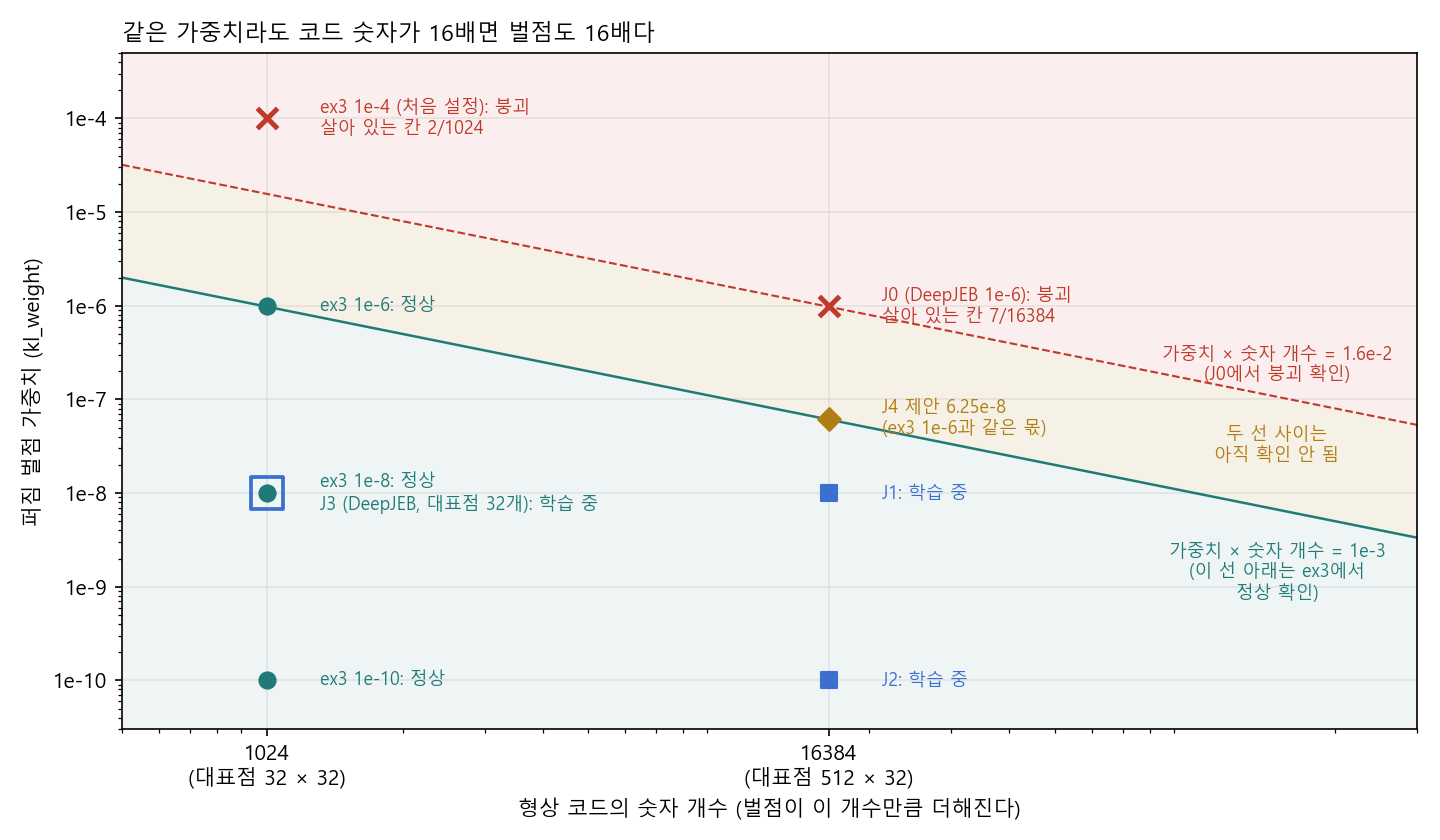
\includegraphics[width=0.78\textwidth]{figures/fig_kl_budget.png}
\caption{퍼짐 벌점 지도. 가로축은 형상 코드의 숫자 개수, 세로축은 \key{kl_weight}. 청록 실선(곱 $=10^{-3}$) 아래는 ex3에서
정상이 확인된 곳, 빨간 점선(곱 $=1.6\times10^{-2}$)은 J0에서 붕괴가 확인된 곳이다. 두 선 사이는 아직 확인하지 않았다.
J4는 ex3의 $10^{-6}$과 같은 곱이 되도록 계산한 제안값이다.}
\label{fig:klbudget}
\end{figure}

\begin{figure}[htbp]
\wide{17.5cm}{figures/fig_collapse.png}
\caption{모든 1단계 실험의 학습 기록(DeepJEB J1--J3는 500바퀴 끝까지). (a) 살아 있는 칸의 비율(로그 눈금).
ex3 처음 설정(빨강)은 흔들림을 키우기 시작한 직후 0으로 떨어진다. 55바퀴에 694개였다가 60바퀴에 12개, 65바퀴에 0개가 되었다.
DeepJEB J0(주황)는 50--150바퀴 구간 내내 줄어 150바퀴 1518개(9\%), 160바퀴 564개(3\%), 200바퀴 43개가 되었다. (b) 점검용 형상의 부호 거리 오차. J0는 75바퀴에 0.00228로 가장
낮았다가 160바퀴에 0.0223까지 올랐고, 295바퀴에 0.00473이었다. ex3와 DeepJEB는 데이터가 달라 두 곡선의 높이를 서로 비교하지는 않는다.}
\label{fig:collapse}
\end{figure}

\paragraph{대표점 수를 바꿀 때의 환산표.}
ex3에서 정상이었던 $10^{-6}$(곱 $1.024\times10^{-3}$)과 같은 세기를 유지하려면 \key{kl_weight}를 대표점 수에 반비례하게 줄인다.

\begin{center}\small
\begin{tabular}{r r r}
\toprule
대표점 수 $T$ (\key{latent_tokens}) & 숫자 개수 $T\times32$ & 같은 세기의 \key{kl_weight} \\
\midrule
32 & 1024 & $1\times10^{-6}$ \\
64 & 2048 & $5\times10^{-7}$ \\
128 & 4096 & $2.5\times10^{-7}$ \\
256 & 8192 & $1.25\times10^{-7}$ \\
512 & 16384 & $6.25\times10^{-8}$ \\
\bottomrule
\end{tabular}
\end{center}

ex3에서는 이보다 100배, 10000배 약한 벌점($10^{-8}$, $10^{-10}$)도 정상이었고 결과도 비슷하거나 조금 나았다(\S\ref{sec:results}).
즉 ``벌점이 세면 무너지고, 약한 쪽으로는 넓은 범위가 괜찮다''. 헷갈리면 약한 쪽을 고르는 편이 안전하다.

% ======================================================================
\section{2단계: 생성 모델}
\label{sec:fm}

\subsection{잡음에서 형상 코드까지 50걸음}

생성 모델은 한 번에 답을 내지 않는다. 난수 표(잡음, 크기 $T\times32$)에서 출발해 50걸음으로 나눠 조금씩 형상 코드 쪽으로
옮긴다(그림~\ref{fig:flow}). 매 걸음마다 생성 모델에게 ``지금 위치, 지금까지 온 정도 $t$(0에서 1), 조건''을 주면
``이쪽으로 가라''는 이동 방향을 돌려준다. 그 방향으로 1/50만큼 움직이고 다시 묻는다.
\[
z \;\leftarrow\; z + \tfrac{1}{50}\; v(z,\; t,\; \text{조건}), \qquad t = 0, \tfrac{1}{50}, \tfrac{2}{50}, \dots, \tfrac{49}{50}
\]
여기서 $z$는 지금 위치(만들어지는 중인 형상 코드)이고, $v$는 생성 모델이 돌려준 이동 방향이다. $\leftarrow$는 ``왼쪽 값을 오른쪽 계산 결과로 바꾼다''는 뜻이다.
걸음 수는 \key{ode_steps 50}이다. 매 걸음이 똑같이 계산되고 도중에 난수를 섞지 않으므로,
\textbf{같은 잡음 + 같은 조건이면 언제나 같은 형상}이 나온다. 그래서 \key{seed}로 잡음을 고정하면 결과를 똑같이 다시 만들 수 있다.

\subsection{무엇을 배우나}

학습할 때는 학습용 형상의 코드(요약부의 평균값) 하나와 잡음 하나를 곧은 선으로 잇고, 그 선 위 한 점
$z_t=(1-t)\cdot\text{잡음}+t\cdot\text{코드}$를 뽑는다. 이 점에서 가야 할 방향은 ``코드 $-$ 잡음''이다. 생성 모델은 이 방향을
맞히도록 배운다. 수많은 쌍을 보면서 배우므로, 나중에는 처음 보는 잡음에서 출발해도 그럴듯한 코드로 가는 길을 안다.

생성 모델이 보는 코드는 요약부의 \emph{평균값}(흔들림 없음)이고, 칸마다 학습용 형상들의 평균을 빼고 표준편차로 나눠
크기를 맞춘 값이다. 생성이 끝나면 이 변환을 거꾸로 해서 복원부에 넣는다.

\begin{figure}[htbp]
\centering
\begin{tikzpicture}[scale=1.0]
\pgfmathsetseed{7}
% noise cloud
\fill[gray!12] (0,0) ellipse (1.7 and 1.5);
\foreach \k in {1,...,70} { \fill[gray!70] ({1.4*(rand)}, {1.2*(rand)}) circle (1.1pt); }
\node[font=\small, align=center] at (0,-1.95) {잡음\\(평균 0, 퍼짐 1인 난수)};
% data cloud: three clusters
\begin{scope}[shift={(8.2,0)}]
\fill[orange!12] (0,0) ellipse (1.9 and 1.6);
\foreach \k in {1,...,22} { \fill[orange!80!black] ({-0.7+0.35*(rand)}, {0.6+0.3*(rand)}) circle (1.1pt); }
\foreach \k in {1,...,22} { \fill[orange!80!black] ({0.6+0.35*(rand)}, {0.5+0.35*(rand)}) circle (1.1pt); }
\foreach \k in {1,...,22} { \fill[orange!80!black] ({0.0+0.45*(rand)}, {-0.7+0.3*(rand)}) circle (1.1pt); }
\node[font=\small, align=center] at (0,-1.95) {학습용 형상 코드\\(칸마다 크기를 맞춤)};
\end{scope}
% straight training pair
\draw[dashed, gray!70!black, thick] (-0.5,0.7) -- (7.5,0.6);
\node[font=\footnotesize, gray!40!black, align=center, anchor=south] at (4.1,1.7) {학습: 잡음과 코드를 곧은 선으로 잇고\\그 위의 점에서 ``코드 $-$ 잡음'' 방향을 맞히게 함};
% generation path with 50 steps
\coordinate (A) at (0.6,-0.5);
\coordinate (B) at (8.2,-0.72);
\draw[redx, very thick, -{Stealth[length=3mm]}] (A) .. controls (3,-1.9) and (5.5,-1.4) .. (B);
\foreach \s in {0,0.1,...,1.0} {
  \pgfmathsetmacro{\u}{1-\s}
  \fill[redx] ({\u*\u*\u*0.6 + 3*\u*\u*\s*3 + 3*\u*\s*\s*5.5 + \s*\s*\s*8.2}, {\u*\u*\u*(-0.5) + 3*\u*\u*\s*(-1.9) + 3*\u*\s*\s*(-1.4) + \s*\s*\s*(-0.72)}) circle (1.6pt);
}
\fill[black] (A) circle (2.2pt);
\node[font=\footnotesize, redx, align=center] at (4.1,-2.95) {생성: 이동 방향을 물어 1/50씩 50걸음 이동 (점은 5걸음마다)};
\node[font=\footnotesize, anchor=north east, fill=white, inner sep=1.5pt, rounded corners=1pt] at ($(A)+(-0.08,-0.1)$) {출발 잡음};
\end{tikzpicture}
\caption{2단계 생성 모델이 하는 일. 학습 때는 잡음과 실제 코드를 곧은 선으로 이어 ``가야 할 방향''을 가르친다(회색 점선).
생성 때는 새 잡음에서 출발해 매 걸음 방향을 물어 50걸음에 걸쳐 코드가 모인 곳으로 간다(빨간 선).
그림의 점 구름은 설명을 위한 가상 예시다.}
\label{fig:flow}
\end{figure}

\subsection{조건, 빈 조건, 조건 강조 배율}

\paragraph{조건.} 조건은 형상에서 직접 잴 수 있는 숫자다. ex3는 상자 크기 3개(형상을 딱 맞게 감싸는 상자의 x, y, z 길이, \key{bbox_x}, \key{bbox_y}, \key{bbox_z}),
부피(\key{volume}), 표면적(\key{area}) 5개를, DeepJEB는 부피와 표면적 2개를 쓴다(\key{condition_names}). 조건값도 학습용 형상들의
평균과 표준편차로 크기를 맞춘 뒤, 평균에서 표준편차의 5배($\pm5$) 넘게 벗어난 값은 잘라낸다(\key{condition_clip 5}).
학습용 형상에서 거의 변하지 않는 조건(표준편차가 \key{min_condition_std 0.00001}보다 작음)이 있으면 학습이 오류로 멈추므로, 그런 조건은 \key{condition_names}에서 빼야 한다.
ex3에는 너트 종류(육각, 잠금 등)를 나타내는 값도 데이터에 들어 있지만 \emph{조건으로는 쓰지 않는다}. 평가할 때 종류별로 나눠 보는 데만 쓴다.

\paragraph{빈 조건.} 학습 중 20\%는 조건을 모두 지우고 ``조건 없음'' 표시를 넣는다(\key{cond_dropout 0.2}, \key{cond_dropout_mode all}).
그래서 한 모델로 조건 없는 생성도, 조건 있는 생성도 할 수 있다.

\paragraph{조건 강조 배율.} 조건 있는 방향과 조건 없는 방향을 둘 다 계산해 차이를 키울 수 있다.
\[
v = v_{\text{빈 조건}} + s\,\bigl(v_{\text{조건}} - v_{\text{빈 조건}}\bigr), \qquad s=\key{cfg_scale}
\]
$s=1$이면 조건 있는 방향 그대로다. $s>1$이면 조건 쪽으로 더 세게 민다. 치수는 더 정확해지지만 모양은 나빠질 수 있다.
ex3에서 $s=2$는 부피 오차를 줄였지만 한 조각 비율을 떨어뜨렸다(\S\ref{sec:cond}).
\texttt{methods/SDFFlow/CLAUDE.md}에 따르면 이전 DeepJEB 실험에서는 $s=3$이 부피 오차를 2.5배 키웠다(8.5\%$\rightarrow$21.2\%). 기본값 1을 권한다.

\paragraph{생성 모델의 크기.} 같은 계산 단계 8개를 차례로 거치고(\key{fm_blocks 8}), 각 단계는 대표점마다 숫자 256개를 다루며(\key{fm_hidden 256})
대표점끼리 8가지 관점으로 정보를 나눈다(\key{fm_heads 8}). 진행 정도 $t$와 조건은 숫자 128개로 바뀌어(\key{fm_cond_hidden 128})
각 단계의 값을 몇 배로 키우고 얼마만큼 더할지를 정하는 데 쓰인다(\key{fm_arch dit}). 이 조절값은 처음에 0에서 시작하므로,
학습 초반에는 각 단계가 입력을 그대로 넘긴다.

% ======================================================================
\section{형상 코드에서 STL까지}
\label{sec:mesh}

\begin{figure}[htbp]
\centering
\begin{tikzpicture}[
  b/.style={draw, rounded corners=2pt, align=center, font=\small, minimum height=1.25cm, inner sep=3pt, text width=2.6cm},
  arr/.style={-{Stealth[length=2mm]}, thick}, node distance=0.42cm]
\node[b, fill=orange!18] (c) {형상 코드\\$T\times32$};
\node[b, fill=blue!6, right=of c] (g) {$128^3$ 격자 점마다\\부호 거리 계산\\(약 210만 점)};
\node[b, fill=blue!6, right=of g] (m) {값이 0인 면을\\삼각형으로 추출};
\node[b, fill=yellow!20, right=of m] (k) {조각 수를 셈\\\key{body_count_raw}\\로 기록};
\node[b, fill=red!10, right=of k] (s) {\textbf{가장 큰 조각만}\\STL로 저장};
\draw[arr] (c) -- (g); \draw[arr] (g) -- (m); \draw[arr] (m) -- (k); \draw[arr] (k) -- (s);
\node[draw=redx, thick, rounded corners, fill=red!3, font=\small, align=left, text width=13.5cm, anchor=north] (w) at ($(c.south west)!0.5!(s.south east)+(0,-0.5)$)
{\textbf{주의:} 마지막 단계는 코드에 고정되어 있다(\key{mesh_extraction.sdf_grid_to_mesh(..., keep_largest=True)}).
config key가 아니므로 끌 수 없다. 떨어진 조각이 있어도 \textbf{STL에는 보이지 않는다}.
떨어진 조각은 실행 기록이나 결과 요약에 남는 \key{body_count_raw}로 확인해야 한다.};
\end{tikzpicture}
\caption{형상 코드에서 STL을 만드는 과정. 격자 해상도는 \key{mc_resolution 128}. 격자 한 칸은 상자 폭 2의 1/127, 약 0.016이다.
이보다 얇은 벽이나 틈은 격자 단계에서 이미 사라지거나 끊길 수 있다.}
\label{fig:mesh}
\end{figure}

그림~\ref{fig:mesh}의 마지막 단계 때문에, 예전에 \texttt{junk/}로 가져온 보간 STL에서는 떨어진 조각이 보이지 않았다.
이 문서의 모든 조각 수는 가장 큰 조각만 남기기 \emph{전의} 값(\key{body_count_raw}, 또는 같은 격자에서 따로 센 값)이다.

% ======================================================================
\section{config 작성법}
\label{sec:config}

\subsection{기본 문법과 실행}

\begin{itemize}
\item 한 줄에 ``key 값'' 하나. 값이 여러 개면 쉼표로 나눈다(예: \key{condition_names volume, area}).
\item \texttt{\%} 뒤는 주석이다. 같은 key를 두 번 쓰면 오류다. 파일 맨 앞에 BOM(보이지 않는 표시 문자)이 있으면 오류다.
\item 경로가 아닌 글자 값은 소문자로 바뀌어 읽힌다. 경로는 적은 그대로 읽힌다.
\item 무엇을 할지(\key{mode})는 명령줄이 아니라 config 안에 적는다.
\item 실행은 AI-CAE4ALL 폴더 맨 위(\texttt{AI\_CAE4ALL\_main.py}가 있는 곳)에서 한다. 프로그램은 \texttt{methods/SDFFlow/}에서 돌기 때문에 경로는
\texttt{../../dataset/...}, \texttt{../../output/...}처럼 적는다.
\end{itemize}

\begin{Verbatim}[fontsize=\small, frame=single, framesep=2mm]
# 검사만 (문제를 한꺼번에 모두 보여 줌)
python AI_CAE4ALL_main.py --config <config 파일> --check
# 실제로 실행될 명령만 보여 주기
python AI_CAE4ALL_main.py --config <config 파일> --dry-run
# 검사를 통과하면 바로 실행
python AI_CAE4ALL_main.py --config <config 파일>
# 필수 key 목록 보기
python AI_CAE4ALL_main.py --describe sdfflow
\end{Verbatim}
\noindent 예를 들어 ex3 학습 config는 \path{configs/SDFFlow/geometry_generation/ex3/baseline/config_train_sdfflow.txt}이다.

\subsection{모드와 꼭 적어야 하는 key}

무엇을 할지는 \key{mode}로 정하고, 모드마다 꼭 적어야 하는 key가 다르다(표~\ref{tab:modes}).

\begin{table}[htbp]
\centering\small
\begin{tabularx}{\textwidth}{l L L}
\toprule
\key{mode} & 하는 일 & 꼭 적어야 하는 key \\
\midrule
\key{train} & 1단계 $\rightarrow$ 2단계 차례로 학습. \key{train_vae}, \key{train_fm}은 한 단계만 &
\key{dataset_dir}, \key{output_dir}, \key{vae_modelpath}, \key{fm_modelpath}, \key{latent_tokens}, \key{latent_dim}, \key{decoder_type}, \key{decoder_hidden}, \key{decoder_layers}, \key{encoder_dim}, \key{encoder_heads}, \key{encoder_blocks}, \key{num_encoder_points}, \key{num_query_points}, \key{fm_hidden}, \key{fm_blocks}, \key{fm_cond_hidden}, 두 단계의 바퀴 수·한 번에 보는 형상 수·학습 속도 \\
\key{sample} & 새 형상 생성 & \key{vae_modelpath}, \key{fm_modelpath}, \key{output_dir}, \key{num_samples}, \key{seed}, \key{ode_steps}, \key{mc_resolution} \\
\key{reconstruct} & 형상 하나를 코드로 줄였다가 복원 & \key{vae_modelpath}, \key{input_mesh}, \key{output_dir}, \key{mc_resolution} \\
\key{interpolate} & 두 생성 형상 사이 섞기, 또는 조건 옮기기 & \key{vae_modelpath}, \key{fm_modelpath}, \key{output_dir}, \key{seed}, \key{source_num_samples}, \key{sample_index_a}, \key{ode_steps}, \key{mc_resolution}, 그리고 방식에 따라 \key{sample_index_b} 또는 \key{cond_values_a}·\key{cond_values_b} \\
\key{evaluate} & 점검용·시험용 형상의 복원 성능 등을 숫자로 평가 & \key{vae_modelpath}, \key{dataset_dir}, \key{output_dir} \\
\key{optimize} & 생성 $\rightarrow$ 격자 생성 $\rightarrow$ 구조 해석 $\rightarrow$ 탐색을 묶은 설계 반복 & \texttt{methods/SDFFlow/CLAUDE.md} 참고 \\
\bottomrule
\end{tabularx}
\caption{SDFFlow 모드와 필수 key(\texttt{cae\_suite/specs/sdfflow.py} 기준). 필수 key가 빠지면 \key{--check}가 알려 준다.}
\label{tab:modes}
\end{table}

\subsection{학습 config: key별 의미와 정하는 법}

표~\ref{tab:trainkeys}는 학습 config의 주요 key를 ex3와 DeepJEB(\texttt{ex1}) 파일의 실제 값과 함께 정리한 것이다.
\key{model}, \key{mode}, \key{parallel_mode}, \key{fm_num_workers}와 학습 중 그림용 설정(\key{vae_num_test_shapes}, \key{vae_mc_resolution_test}, \key{fm_num_test_shapes}, \key{fm_mc_resolution_test})은 표에서 뺐다.
DeepJEB 값은 ex3와 다른 곳만 적었다. 파일 원문은 부록~\ref{app:config}에 있다.

{\small
\begin{longtable}{>{\raggedright\arraybackslash}p{4.4cm} >{\raggedright\arraybackslash}p{1.9cm} >{\raggedright\arraybackslash}p{2.1cm} >{\raggedright\arraybackslash}p{5.6cm}}
\caption{학습 config key. ``ex3''는 ex3 학습 config(원문은 부록~\ref{app:config}), ``DeepJEB''는 경로의 \texttt{ex3}만 \texttt{ex1}로 바꾼
같은 이름의 파일(현재 작업본)이다. 빈칸은 ex3와 같음.}\label{tab:trainkeys}\\
\toprule
key & ex3 & DeepJEB & 뜻과 정하는 법 \\
\midrule
\endfirsthead
\toprule
key & ex3 & DeepJEB & 뜻과 정하는 법 \\
\midrule
\endhead
\bottomrule
\endfoot
\multicolumn{4}{l}{\textbf{데이터}}\\
\key{dataset_dir} & \key{ex3_mcb.h5} & \key{ex1_deepjeb.h5} & 학습 데이터 파일 \\
\key{split_by_parent} & False & True & 같은 부모 형상에서 나온 형제를 모두 같은 쪽(학습용/점검용/시험용)에 둔다. DeepJEB는 반드시 True. 아니면 점검용에 학습용 형제가 섞여 성능이 부풀려진다 \\
\key{seed}, \key{split_seed} & 42, 42 & & 난수 고정. 데이터 나누기에도 같은 값이 쓰인다 \\
\key{gpu_ids} & 1 & 7 & 쓸 GPU 번호 \\
\midrule
\multicolumn{4}{l}{\textbf{점 수}}\\
\key{num_encoder_points} & 6144 & & 요약부에 넣는 표면 점 수 \\
\key{num_query_points} & 8192 & & 학습 때 형상마다 부호 거리를 맞춰 볼 점 수. 저장된 점(ex3 81920개, DeepJEB 10240개)에서 뽑는다 \\
\midrule
\multicolumn{4}{l}{\textbf{형상 코드와 요약부}}\\
\key{latent_tokens} & 32 & \textbf{512} & 대표점 수 $T$. 바꾸면 \key{kl_weight}를 다시 계산해야 한다(\S\ref{sec:kl}) \\
\key{latent_dim} & 32 & & 대표점마다 숫자 개수 \\
\key{encoder_query_type} & fps & & 대표점 고르는 법. fps = 서로 가장 멀리 떨어진 점 \\
\key{encoder_dim}, \key{encoder_heads}, \key{encoder_blocks} & 256, 8, 4 & & 요약부가 점마다 다루는 숫자 개수, 관점 수, 반복 횟수 \\
\key{encoder_self_attention} & True & & 대표점끼리 정보를 나눌지 \\
\key{fourier_bands} & 8 & & 사인·코사인 늘리기 단계 수 ($3\rightarrow51$) \\
\midrule
\multicolumn{4}{l}{\textbf{복원부}}\\
\key{decoder_type} & attention & & 질문 점이 대표점을 훑어보는 방식. 대표점이 여러 개면 이것을 쓴다 \\
\key{decoder_hidden}, \key{decoder_layers}, \key{decoder_heads} & 256, 4, 8 & & 복원부가 점마다 다루는 숫자 개수, 층 수, 관점 수 \\
\key{clamp_dist} & 0.1 & & 부호 거리를 자르는 거리 \\
\midrule
\multicolumn{4}{l}{\textbf{퍼짐 벌점과 흔들림}}\\
\key{kl_weight} & 1e-10 & \textbf{1e-6} & 퍼짐 벌점 가중치. \S\ref{sec:kl}의 곱이 $10^{-3}$ 이하가 되게. DeepJEB 파일의 값은 J0에서 붕괴가 확인된 조합이다(\S\ref{sec:recommend}) \\
\key{deterministic_warmup_epochs} & 50 & & 흔들림·벌점 없이 복원만 하는 바퀴 수 \\
\key{posterior_noise_warmup_epochs} & 100 & & 흔들림을 키우는 바퀴 수 \\
\key{posterior_noise_max_scale} & 1 & & 흔들림의 최종 크기(1 = 퍼짐 정도 그대로) \\
\key{kl_warmup_epochs} & 200 & & 벌점을 키우는 바퀴 수 \\
\key{posterior_min_std_rel} & 0.05 & & 흔들림 크기의 하한(숫자 자리별로, 모든 형상·대표점에 걸친 평균값 퍼짐 폭의 5\%) \\
\midrule
\multicolumn{4}{l}{\textbf{오차 항목}}\\
\key{surface_weight}, \key{normal_weight}, \key{eikonal_weight} & 1, 0.1, 0.1 & & 표~\ref{tab:loss} \\
\key{hybrid_grad_points} & 1024 & & 표면·면 방향·기울기 크기를 계산할 점 수 \\
\midrule
\multicolumn{4}{l}{\textbf{조건}}\\
\key{use_conditions} & True & & 조건을 쓸지 \\
\key{condition_names} & \key{bbox_x, bbox_y, bbox_z,} volume, area & volume, area & 조건 목록. 생성할 때 조건값도 이 순서로 적는다 \\
\key{min_condition_std}, \key{condition_clip} & 0.00001, 5 & & 표준편차가 앞의 값보다 작은 조건이 있으면 학습이 오류로 멈춤(\key{condition_names}에서 뺄 것). 뒤의 값은 크기를 맞춘 조건을 자르는 범위 \\
\key{cond_dropout}, \key{cond_dropout_mode} & 0.2, all & & 조건을 지우는 비율과 방식. all = 한꺼번에 모두 지움. per\_dim = 조건마다 따로 지움(생성 때 일부 조건만 \texttt{nan}으로 비워 둘 수 있음) \\
\midrule
\multicolumn{4}{l}{\textbf{생성 모델}}\\
\key{fm_arch} & dit & & 생성 모델 종류 \\
\key{fm_hidden}, \key{fm_blocks}, \key{fm_heads}, \key{fm_cond_hidden} & 256, 8, 8, 128 & & 대표점마다 다루는 숫자 개수, 계산 단계 수, 관점 수, 진행 정도 $t$·조건을 바꾼 숫자 개수 \\
\key{fm_time_sampling} & uniform & & 학습 때 진행 정도 $t$를 고르게 뽑음 \\
\key{ode_steps} & 50 & & 생성 걸음 수 \\
\key{encode_batch_size} & 8 & & 2단계 시작 전 학습용 형상을 코드로 바꿀 때 한 번에 처리하는 형상 수 \\
\midrule
\multicolumn{4}{l}{\textbf{1단계 학습}}\\
\key{vae_training_epochs} & 1000 & \textbf{1500} & 바퀴 수. 700--900이면 충분(\S\ref{sec:epochs}) \\
\key{vae_batch_size} & 8 & & 한 번에 보는 형상 수 \\
\key{vae_learningr}, \key{vae_weight_decay} & 0.0001, 0.0001 & & 학습 속도, 모델 내부 숫자를 조금씩 작게 당기는 정도 \\
\key{vae_warmup_epochs} & 20 & & 학습 속도를 서서히 올리는 바퀴 수 \\
\key{vae_use_amp} & False & & 계산 정밀도 낮추기(속도용). 1단계는 끔 \\
\key{vae_use_ema}, \key{vae_ema_decay} & True, 0.99 & & 학습 중 모델 내부 숫자들의 최근 평균(가중치 평균본)을 따로 들고 있다가 그것을 저장. 값이 덜 흔들린다 \\
\key{vae_val_interval}, \key{vae_test_interval} & 5, 100 & & 점검용 오차를 잴 간격, 그림을 그릴 간격 \\
\key{vae_num_workers} & 2 & & 데이터 읽기 보조 작업 수 \\
\midrule
\multicolumn{4}{l}{\textbf{2단계 학습}}\\
\key{fm_training_epochs} & 500 & & 바퀴 수. 약 700 권장(\S\ref{sec:epochs}) \\
\key{fm_batch_size} & 64 & & 한 번에 보는 코드 수 \\
\key{fm_learningr}, \key{fm_weight_decay} & 0.0001, 0.0001 & & \\
\key{fm_warmup_epochs} & 10 & & \\
\key{fm_use_amp} & True & & 2단계는 켬 \\
\key{fm_use_ema}, \key{fm_ema_decay} & True, 0.99 & & \\
\key{fm_val_interval}, \key{fm_test_interval} & 5, 50 & & \\
\midrule
\multicolumn{4}{l}{\textbf{저장 위치와 기타}}\\
\key{vae_modelpath}, \key{fm_modelpath} & \multicolumn{2}{>{\raggedright\arraybackslash}p{4.4cm}}{\texttt{../../output/.../vae.pth}, \texttt{fm.pth}} & 학습이 끝난 모델 파일 \\
\key{fm_best_modelpath} & \multicolumn{2}{>{\raggedright\arraybackslash}p{4.4cm}}{\texttt{.../fm\_best.pth}} & 2단계 점검용 오차가 가장 낮았던 시점의 파일. 생성에는 이것을 쓴다 \\
\key{output_dir}, \key{pipeline_log_file}, \key{vae_log_file_dir}, \key{fm_log_file_dir} & \multicolumn{2}{>{\raggedright\arraybackslash}p{4.4cm}}{\texttt{../../output/...}} & 결과와 기록. 반드시 AI-CAE4ALL 폴더의 \texttt{output/} 아래 \\
\key{skip_completed_stages} & True & & 이미 끝난 단계는 다시 학습하지 않음 \\
\key{display_testset} & True & & 학습 중 주기적으로 형상 그림을 저장 \\
\end{longtable}
}

\subsection{바퀴 수는 충분한가}
\label{sec:epochs}

\begin{figure}[htbp]
\wide{17.5cm}{figures/fig_epochs.png}
\caption{바퀴 수 점검(ex3). (a) 1단계: 점검용 부호 거리 오차(굵은 선)는 약 500바퀴부터 평탄하고, 가장 좋은 지점은
885(1e-6), 730(1e-8), 625(1e-10)바퀴다. 끝 무렵 학습용 오차(옅은 선)는 0.0022--0.0024, 점검용은 0.0067--0.0071이고 둘 다 평탄하다.
(b) 2단계: 500바퀴 실행은 가장 좋은 지점이 455--499바퀴로, 끝날 때까지 좋아지는 중이었다. 2000바퀴로 늘린 세 실행
(기본 설정, 진행 정도 $t$를 뽑는 방식 변경, 거기에 가중치 평균본을 더 천천히 갱신)은 가장 좋은 지점이 680, 530, 640바퀴였고 그 뒤로는 나아지지 않았다.}
\label{fig:epochs}
\end{figure}

\begin{itemize}
\item \textbf{1단계}: 1000바퀴는 충분하다. 700--900바퀴면 된다. 500바퀴 이후로는 점검용 오차가 거의 변하지 않는다.
학습용 오차(학습 중 흔들림을 섞은 채로 잰 값)는 점검용의 약 1/3에서 역시 평탄하다. 이 차이는 바퀴를 늘려서 줄어드는 것이 아니고,
대부분 오차가 유난히 큰 소수의 잠금·캐슬 너트에서 온다(점검용/학습용 오차 중앙값은 같고 평균만 3.6배, \S\ref{sec:castle}). DeepJEB J1--J3도 500바퀴면 충분했다.
400바퀴에서 500바퀴까지 점검용 오차가 J1 1.4\%, J2 1.6\%, J3 0.5\%만 더 내려갔다.
\item \textbf{2단계}: 500바퀴는 조금 모자라다. 약 700바퀴로 늘리고 \key{fm_best.pth}를 쓰기를 권한다. 2000바퀴까지 늘려도 이득이 없었다.
\end{itemize}

\subsection{생성(sample) config}

\begin{Verbatim}[fontsize=\small, frame=single, framesep=2mm]
model                sdfflow
mode                 sample
seed                 42
vae_modelpath        ../../output/.../vae.pth
fm_modelpath         ../../output/.../fm_best.pth     % 가장 좋았던 시점 파일
output_dir           ../../output/.../samples
num_samples          209
ode_steps            50
mc_resolution        128
cfg_scale            1                                % 조건 강조 배율, 기본 1
% 조건을 줄 때만 (condition_names 순서, 학습 데이터와 같은 단위):
% cond_values        0.35, 4.1
condition_ood_policy error                            % error | warn | clamp
max_condition_z      3
\end{Verbatim}

\begin{itemize}
\item \key{cond_values}를 적지 않으면 빈 조건으로 만든다. 적으면 \key{condition_names} 순서로 모든 값을 적는다.
일부만 \texttt{nan}(``값 없음''이라는 뜻으로 적는 글자)으로 비워 두려면 2단계를 \key{cond_dropout_mode per_dim}으로 학습했어야 한다.
\item 요청한 조건이 학습 데이터 평균에서 표준편차의 3배(\key{max_condition_z 3}) 넘게 벗어나면, \key{condition_ood_policy}에 따라
멈추거나(\texttt{error}), 경고만 하거나(\texttt{warn}), 경계값으로 잘라서(\texttt{clamp}) 만든다.
\item 위 예의 \key{cond_values} 숫자는 형식을 보여 주는 예시일 뿐이다.
\end{itemize}

\subsection{보간(interpolate) config}
\label{sec:interp-config}

\key{interpolation_space}로 세 가지 방식을 고른다.

\begin{description}[leftmargin=1.2em]
\item[\key{slerp_noise} (기본).] 생성 모델의 잡음 두 줄을 원호를 따라 섞은 뒤 50걸음 생성한다. 여기서 잡음 ``한 줄''은 형상 하나를 만드는 잡음이다
(seed 42라면 0번 줄이 \texttt{sample\_42\_000.stl}을 만든다. 두 줄은 \key{sample_index_a}, \key{sample_index_b}번째 줄).
숫자가 많은 잡음은 전체 크기(모든 숫자를 제곱해 더한 값)가 거의 일정한데, 두 잡음을 직선으로 섞으면 중간에서 이 크기가 작아져
``평범하지 않은 잡음''이 된다. 원호로 섞으면 크기가 유지된다. 두 끝은 원래 생성 형상과 똑같다.
\item[\key{lerp_latent} (예전 방식).] 두 생성 형상의 코드(칸마다 크기를 맞춘 값)를 직선으로 섞는다.
\item[\key{cond_sweep}.] 잡음 한 줄을 고정하고 조건만 \key{cond_values_a}에서 \key{cond_values_b}까지 \key{sweep_steps}칸(기본 5, 2 이상)에 걸쳐
직선으로 옮긴다. 결과는 \texttt{sample\_<seed>\_sweep\_<k>.stl}로 저장된다. 조건 있는 2단계 모델이 필요하다.
\end{description}

\begin{Verbatim}[fontsize=\small, frame=single, framesep=2mm]
% (가) 두 생성 형상 사이 섞기
mode                 interpolate
interpolation_space  slerp_noise
seed                 42
source_num_samples   209        % sample 실행의 num_samples와 같게
sample_index_a       0          % 그 실행의 sample_42_000.stl
sample_index_b       1          % 그 실행의 sample_42_001.stl
alpha                0.5        % 한 번 실행에 섞는 비율 하나
ode_steps            50
cfg_scale            1
mc_resolution        128

% (나) 조건만 옮기기 (DeepJEB: volume, area 순서)
mode                 interpolate
interpolation_space  cond_sweep
seed                 42
source_num_samples   209
sample_index_a       0          % 고정할 잡음 줄
cond_values_a        <부피 A>, <면적 A>
cond_values_b        <부피 B>, <면적 B>
sweep_steps          9
cfg_scale            1
\end{Verbatim}

제약과 주의점은 다음과 같다.
\begin{itemize}
\item \key{slerp_noise}와 \key{lerp_latent}는 \textbf{조건 없는 섞기만} 된다. \key{cond_values}를 적으면 프로그램이 멈춘다.
조건을 쓰려면 \key{cond_sweep}을 쓴다.
\item 한 번 실행에는 비율(\key{alpha})을 하나만 쓴다. 두 끝과 중간 하나, 그리고 세 형상을 나란히 그린 그림이 저장된다.
비율 11개를 보려면 11번 실행한다.
\item 끝점은 \emph{생성된} 형상이다. \textbf{실제 데이터 형상 두 개 사이를 섞는 기능은 지금 없다}. 이 문서의 실제 형상 사이 보간(\S\ref{sec:paths})은
따로 만든 평가 프로그램으로 돌렸다.
\item 끝점을 \key{mode sample} 결과와 똑같이 맞추려면 \key{seed}와 \key{source_num_samples}를 그 실행의 \key{seed}, \key{num_samples}와 같게 둔다.
만든 잡음 개수가 다르면 앞쪽 번호의 잡음이 같게 나온 적은 있지만 보장되지는 않는다.
\end{itemize}

\subsection{복원(reconstruct)과 평가(evaluate) config}

\begin{Verbatim}[fontsize=\small, frame=single, framesep=2mm]
mode                      reconstruct
vae_modelpath             ../../output/.../vae.pth
input_mesh                <복원할 STL 경로>
output_dir                ../../output/.../recon
mc_resolution             128
latent_refine_steps       1000     % 0이면 끔. 복원 품질이 목적이면 켬
latent_refine_lr          0.01
latent_refine_prior_weight 0

mode                      evaluate
vae_modelpath             ../../output/.../vae.pth
dataset_dir               ../../dataset/geometry_generation/ex1_deepjeb.h5
output_dir                ../../output/.../eval
split_seed                42
split_by_parent           True     % 학습 때와 반드시 같게
eval_task                 reconstruction
eval_split                test     % train | val | test
eval_num_shapes           0        % 0 = 전부
\end{Verbatim}

\key{latent_refine_steps}는 요약부가 낸 코드를 출발점으로, 복원 결과가 입력 형상과 더 맞도록 코드를 직접 1000번 고치는 기능이다.
ex3에서 이렇게 하면 표면 평균 거리가 ``정답 형상을 같은 격자로 뽑았을 때의 표면 평균 거리''의 1.04--1.09배까지 내려갔다
(kl 1e-6 점검용 중앙값 0.0069 $\rightarrow$ 0.0064). 즉 복원부는 충분히 좋고, 부족한 것은 요약부다.
대신 고친 코드는 요약부가 내는 코드의 퍼짐 범위에서 59--61\% 벗어나므로, \textbf{고친 코드를 2단계 학습에 넣으면 안 된다}.

\subsection{자주 하는 실수 점검표}

\begin{enumerate}
\item \key{latent_tokens}를 바꾸고 \key{kl_weight}를 그대로 둠 $\rightarrow$ 벌점이 대표점을 늘린 배수만큼 세짐(32 $\rightarrow$ 512면 16배). DeepJEB 파일의 512 / 1e-6이 이 경우다.
\item STL만 보고 떨어진 조각이 없다고 판단함 $\rightarrow$ \key{body_count_raw}를 볼 것(\S\ref{sec:mesh}).
\item DeepJEB에서 \key{split_by_parent False} $\rightarrow$ 형제 형상이 점검용에 섞임. \key{mode evaluate}도 학습 때와 같은 값으로.
\item 250바퀴 전의 점검용 오차로 실험을 비교함 $\rightarrow$ 흔들림·벌점이 커지는 중이라 비교가 안 됨.
\item 보간 끝점이 sample 결과와 다름 $\rightarrow$ \key{source_num_samples}를 \key{num_samples}와 같게.
\item \key{slerp_noise}에 \key{cond_values}를 적음 $\rightarrow$ 멈춤. 조건 섞기는 \key{cond_sweep}.
\item \key{cfg_scale}을 크게 둠 $\rightarrow$ 치수는 맞아도 모양이 나빠짐. 기본 1, 치수가 꼭 맞아야 할 때만 2.
\item \key{fm.pth}(마지막 시점)로 생성 $\rightarrow$ \key{fm_best.pth} 권장.
\item 조건값의 순서나 단위가 틀림 $\rightarrow$ \key{condition_names} 순서, 학습 데이터와 같은 단위.
\item 코드를 고친 복원 결과(\key{latent_refine_steps} $>0$)를 2단계 학습 데이터로 씀 $\rightarrow$ 쓰지 말 것.
\item 실행 전에 \key{--check}를 안 돌림 $\rightarrow$ 필수 key 누락, 허용되지 않는 값, 경로 오류를 한 번에 잡아 준다.
\end{enumerate}

% ======================================================================
\section{실험 방법}
\label{sec:method}

\subsection{데이터}

두 데이터의 차이는 표~\ref{tab:data}에 정리했다. 실제 형상은 ex3가 그림~\ref{fig:dataex3}, DeepJEB가 그림~\ref{fig:datajeb}에 있다.

\begin{table}[htbp]
\centering\small
\begin{tabularx}{\textwidth}{l L L}
\toprule
 & ex3 (MCB 너트) & DeepJEB (브래킷) \\
\midrule
형상 수 & 1305 (학습용 1044 / 점검용 130 / 시험용 131) & 2138, 부모 형상 263개 \\
종류 & 5종: 육각 824, 잠금 196, 캐슬 181, 홈 59, 사각 45 & 1종 (부모 421번은 형제 15개) \\
\key{split_by_parent} & False (부모 정보 없음) & True \\
놓인 방향 & 제각각 (세움 / 누움 / 비스듬, 그림~\ref{fig:orient}) & 모두 같음 \\
조건 & 상자 크기 3개, 부피, 면적 (5개) & 부피, 면적 (2개, 실질적으로 약 1.5개 몫) \\
형상당 저장된 부호 거리 점 & 81920 & 10240 (표면 근처 8192 + 고르게 2048) \\
\bottomrule
\end{tabularx}
\caption{두 데이터의 차이. DeepJEB는 부피와 면적이 서로 강하게 함께 움직여서 조건 두 개가 사실상 1.5개 정도의 정보만 준다.}
\label{tab:data}
\end{table}

\begin{figure}[htbp]
\wide{17cm}{figures/fig_data_ex3.png}
\caption{ex3의 5종 너트. 종류마다 가장 흔한 방향과 다른 방향으로 놓인 실제 형상을 하나씩 보였다. 같은 종류라도 세워진 것과 눕혀진 것이 섞여 있다.}
\label{fig:dataex3}
\end{figure}

\begin{figure}[htbp]
\wide{17cm}{figures/fig_data_jeb.png}
\caption{DeepJEB 브래킷. 위 줄은 부모 421번의 형제 5개(152, 229, 233, 482, 61번), 아래 줄은 서로 다른 부모 5개(290, 86, 142, 513, 14번)에서 하나씩.
형제끼리는 같은 계열의 조금씩 다른 변형이다. 모든 형상이 같은 방향으로 놓여 있다.}
\label{fig:datajeb}
\end{figure}

\subsection{놓인 방향}
\label{sec:orient-data}

너트의 구멍 축 방향을 표면 점 분포의 세 주축으로 구했다. 세 주축 가운데 길이가 나머지 둘과 가장 다른 축을 구멍 축으로 보고,
그 축이 x, y, z 어느 것과도 $18^\circ$ 넘게 어긋나면 ``비스듬''으로 셌다(그림~\ref{fig:orient}).
ex3 1305개는 z 방향(세움) 742, x 방향(누움) 330, y 방향(누움) 128, 비스듬 105개다. 육각 너트의 28\%, 홈 너트의 92\%가
x 방향으로 누워 있고, 캐슬 너트는 비스듬이 75개다. DeepJEB는 2138개가 거의 모두(축마다 2137--2138개) 가장 긴 축이 y, 중간 축이 x, 가장 짧은 축이 z로 같다.

\begin{figure}[htbp]
\wide{17.5cm}{figures/fig_orient.png}
\caption{놓인 방향. (a) ex3 종류별 구멍 축 방향(z / x / y / 비스듬): 육각 484 / 229 / 99 / 12, 잠금 144 / 28 / 9 / 15,
캐슬 87 / 8 / 11 / 75, 홈 1 / 54 / 4 / 0, 사각 26 / 11 / 5 / 3. (b) DeepJEB는 모든 형상의 세 주축이 같다.}
\label{fig:orient}
\end{figure}

\subsection{비교한 모델}

ex3에서 1단계의 \key{kl_weight}만 바꾼 네 모델을 비교했다. 처음 설정 1e-4(붕괴), 1e-6, 1e-8, 1e-10.
나머지 설정은 모두 같고, 각 모델마다 2단계를 500바퀴 학습했다. 한 모델 안에서 같은 잡음은 늘 같은 형상을 만들지만,
모델이 서로 다르므로 \emph{같은 잡음이라도 모델마다 끝점 형상이 다르다}.

\subsection{섞기 경로 7가지}
\label{sec:paths}

섞는 방법은 네 종류이고(그림~\ref{fig:paths}), 끝점과 조건을 달리해 경로 7묶음을 만들었다(표~\ref{tab:paths}).

\begin{figure}[htbp]
\centering
\begin{tikzpicture}[
  b/.style={draw, rounded corners=2pt, align=center, font=\footnotesize, minimum height=0.95cm, inner sep=2pt, text width=2.05cm},
  lab/.style={font=\footnotesize, anchor=west, align=left, text width=2.9cm},
  arr/.style={-{Stealth[length=1.8mm]}, thick}, node distance=0.3cm]
% row 1
\node[lab] (l1) at (0,0) {\textbf{(가) 잡음 섞기}\\D1, D1c};
\node[b, fill=gray!12, right=0.1cm of l1] (a1) {잡음 A, B};
\node[b, fill=gray!12, right=of a1] (a2) {원호 섞기\\비율 $\alpha$};
\node[b, fill=red!8, right=of a2] (a3) {생성 50걸음\\(빈 조건 / 고정 조건)};
\node[b, fill=teal!12, right=of a3] (a4) {복원부};
\node[b, fill=blue!6, right=of a4] (a5) {형상};
\draw[arr] (a1)--(a2); \draw[arr] (a2)--(a3); \draw[arr] (a3)--(a4); \draw[arr] (a4)--(a5);
% row 2
\node[lab] (l2) at (0,-1.6) {\textbf{(나) 코드 직선 섞기}\\SAME / CROSS\\lerp\_mu};
\node[b, fill=blue!6, right=0.1cm of l2] (b1) {실제 형상 A, B};
\node[b, fill=teal!12, right=of b1] (b2) {요약부 평균};
\node[b, fill=orange!18, right=of b2] (b3) {직선 섞기\\비율 $\alpha$};
\node[b, fill=teal!12, right=of b3] (b4) {복원부};
\node[b, fill=blue!6, right=of b4] (b5) {형상\\(생성 모델\\안 씀)};
\draw[arr] (b1)--(b2); \draw[arr] (b2)--(b3); \draw[arr] (b3)--(b4); \draw[arr] (b4)--(b5);
% row 3
\node[lab] (l3) at (0,-3.2) {\textbf{(다) 거꾸로 걸어}\\\textbf{잡음 찾아 섞기}\\inv\_null / inv\_cond};
\node[b, fill=blue!6, right=0.1cm of l3] (c1) {실제 형상 A, B\\$\rightarrow$ 요약부 평균};
\node[b, fill=red!8, right=of c1] (c2) {생성 모델을\\거꾸로 50걸음\\$\rightarrow$ 잡음 A$'$, B$'$};
\node[b, fill=gray!12, right=of c2] (c3) {원호 섞기\\비율 $\alpha$};
\node[b, fill=red!8, right=of c3] (c4) {앞으로 50걸음\\(빈 조건 / 조건도\\직선으로 옮김)};
\node[b, fill=blue!6, right=of c4] (c5) {복원부\\$\rightarrow$ 형상};
\draw[arr] (c1)--(c2); \draw[arr] (c2)--(c3); \draw[arr] (c3)--(c4); \draw[arr] (c4)--(c5);
% row 4
\node[lab] (l4) at (0,-4.8) {\textbf{(라) 조건만 옮기기}\\CSWEEP\\(\key{cond_sweep})};
\node[b, fill=gray!12, right=0.1cm of l4] (d1) {잡음 1개 고정};
\node[b, fill=yellow!20, right=of d1] (d2) {조건: A의 조건\\$\rightarrow$ B의 조건\\직선 이동};
\node[b, fill=red!8, right=of d2] (d3) {생성 50걸음\\(강조 배율\\1, 2)};
\node[b, fill=teal!12, right=of d3] (d4) {복원부};
\node[b, fill=blue!6, right=of d4] (d5) {형상};
\draw[arr] (d1)--(d2); \draw[arr] (d2)--(d3); \draw[arr] (d3)--(d4); \draw[arr] (d4)--(d5);
\end{tikzpicture}
\caption{평가에 쓴 네 종류의 섞기. (가)는 프로그램의 \key{slerp_noise}와 같다. (나)와 (다)는 실제 형상 두 개 사이를 섞기 위해 따로 만든
평가 프로그램으로 돌렸다(프로그램에 없는 기능). (라)는 프로그램의 \key{cond_sweep}과 같다.
(다)에서 찾은 잡음을 다시 앞으로 걸으면 원래 형상과의 겹침률(두 형상 내부가 겹치는 부피 $\div$ 둘을 합친 부피, 1이면 똑같음) 중앙값이 1.00이라, 거꾸로 걷기 자체는 정확하다.}
\label{fig:paths}
\end{figure}

\begin{table}[htbp]
\centering\small
\begin{tabularx}{\textwidth}{>{\raggedright\arraybackslash}p{2.6cm} L c L >{\raggedright\arraybackslash}p{2.9cm}}
\toprule
이름 & 끝점 & 방법 & 조건 & 개수 \\
\midrule
D1 & 새 잡음 쌍 (seed 7) & (가) & 빈 조건 & 16경로 $\times$ 11비율 \\
D1c & D1의 앞 8쌍과 같은 잡음 & (가) & 쌍마다 점검용 형상 하나의 실제 조건으로 고정 & 8 $\times$ 11 \\
SAME lerp\_mu & 같은 종류의 실제 점검용 형상 쌍 & (나) & --- & 8 $\times$ 11 \\
SAME inv\_null & 같은 쌍 & (다) & 빈 조건 & 8 $\times$ 11 \\
SAME inv\_cond & 같은 쌍 & (다) & 각 끝을 자기 조건으로 거꾸로 걷고, 조건도 직선으로 옮김 & 8 $\times$ 11 \\
CROSS lerp\_mu / inv\_null & 다른 종류의 실제 형상 쌍 & (나) / (다) & --- / 빈 조건 & 8 $\times$ 11 \\
CSWEEP & 잡음 고정, 조건만 A$\rightarrow$B & (라) & 강조 배율 1, 2 & 모델·배율마다 8경로 $\times$ 9비율 \\
\bottomrule
\end{tabularx}
\caption{섞기 경로 목록. 비율 11개는 0, 0.1, …, 1이고, CSWEEP의 9개는 0, 0.125, …, 1이다.
CSWEEP 경로 8개는 SAME 앞 4쌍(육각 443$\rightarrow$938, 잠금 210$\rightarrow$1080, 캐슬 383$\rightarrow$355, 홈 1254$\rightarrow$1246) $\times$ 잡음 2개(seed 11)이다.}
\label{tab:paths}
\end{table}

\subsection{지표}

모든 형상은 $128^3$ 격자에서 가장 큰 조각만 남기기 \emph{전의} 상태로 셌다.

\begin{description}[leftmargin=1.2em]
\item[겹침률.] 두 형상을 같은 $128^3$ 격자에 놓았을 때, 두 형상 내부가 겹친 부피를 둘 중 하나라도 차지한 부피로 나눈 값. 완전히 같으면 1, 전혀 겹치지 않으면 0이다.
\item[한 조각 비율.] 형상이 조각 하나로 나오는 비율. ``중간''은 비율 0.1--0.9의 9칸만 센 것이다. 높을수록 좋다.
\item[추가 조각.] 격자 칸 100개보다 큰 조각의 수에서 1을 뺀 값의 평균. 작은 먼지 같은 조각은 세지 않는다. 낮을수록 좋다.
\item[튐 지수.] 이웃한 두 비율 사이에서 형상 내부가 얼마나 바뀌었는지(1 $-$ 겹침률)를 재고, 그 가운데 최댓값을 중앙값으로 나눈 것.
고르게 변하면 1--2, 한 번에 뒤집히면 커진다. ``튐 $>3$''은 튐 지수가 3을 넘는 경로의 비율이다.
\item[구멍 수 오르내림.] 경로를 따라 가장 큰 조각의 구멍 수가 오르내린 총량이 두 끝의 구멍 수 차이보다 큰 경로의 비율. 구멍이 닫혔다가 다시 뚫리면 여기에 걸린다. 낮을수록 좋다.
\item[조건 오차.] CSWEEP에서, 각 비율에서 요구한 조건값(두 끝 조건의 직선 섞기)과 생성 형상에서 잰 값의 상대 오차. 경로별 중앙값.
\item[부피 순위 상관.] 비율 $\alpha$의 순서와 생성 형상 부피의 순서가 얼마나 같은지(1이면 완전히 같음). 요구 부피가 5\% 넘게 변하는 경로로 계산.
\item[끝점 겹침률.] CSWEEP 끝 형상과 그 조건을 준 실제 형상의 겹침률.
\end{description}

% ======================================================================
\section{ex3 결과}
\label{sec:results}

\subsection{경로 하나를 자세히 보기}

\begin{figure}[htbp]
\wide{17.5cm}{figures/fig_interp_kl.png}
\caption{seed 42 잡음의 0번, 1번 줄을 원호로 섞은 경로(빈 조건). 행은 모델 4개, 열은 섞는 비율 0$\rightarrow$1.
청록은 가장 큰 조각, 빨강은 나머지 조각이다. 칸의 숫자는 프로그램이 기록한 조각 수(\key{body_count_raw})와 가장 큰 조각의 구멍 수다.}
\label{fig:interpkl}
\end{figure}

그림~\ref{fig:interpkl}과 표~\ref{tab:figd}은 프로그램의 기본 보간(\key{slerp_noise}) 경로 하나다.
처음 설정(1e-4)은 비율 0.1--0.8 내내 5--18조각으로 부서지고(0.9에서도 2조각), 떨어진 조각이 표면적의 최대 64.4\%를 차지한다.
예전에 가져온 STL에는 이 가운데 가장 큰 조각만 남아 있었다. 1e-6의 떨어진 조각은 모두 표면적 5\% 미만의 작은 점이고,
1e-8과 1e-10은 거의 없다. 대신 1e-8은 비율 0.1--0.5에서 구멍이 닫힌 판(구멍 수 0)이 되었다가 0.8$\rightarrow$0.9에서 한 번에 육각 너트로
튀고, 1e-10은 0.5$\rightarrow$0.6에서 판에서 캐슬 고리로 튄다.

\begin{table}[htbp]
\centering\small
\begin{tabular}{l l r r r}
\toprule
모델 & 조각 수 (비율 0 $\rightarrow$ 1) & \shortstack[r]{떨어진 조각\\최대 면적} & 튐 지수 & \shortstack[r]{경로 길이\\/ 직선 거리} \\
\midrule
1e-4 (처음) & 1 6 5 5 10 5 8 18 17 2 1 & 64.4\% & 7.6 & 5.81 \\
1e-6 & 1 2 3 1 5 5 3 5 3 5 1 & 4.5\% & 2.7 & 2.21 \\
1e-8 & 1 1 1 1 1 1 1 2 2 1 1 & $<0.1$\% & 12.2 & 2.83 \\
1e-10 & 1 1 1 1 1 1 1 1 1 1 1 & 0 & 3.3 & 1.79 \\
\bottomrule
\end{tabular}
\caption{그림~\ref{fig:interpkl}의 경로 하나(경로 1개뿐). 여기서 튐 지수와 경로 길이는 이웃 STL 사이 표면 평균 거리로 쟀다.
경로 길이 / 직선 거리가 클수록 두 끝 사이를 돌아서 간 것이다.}
\label{tab:figd}
\end{table}

\subsection{여러 경로의 통계}

경로 하나로는 판단할 수 없으므로, 모델마다 표~\ref{tab:paths}의 경로를 모두 돌렸다(표~\ref{tab:four}).

\begin{table}[p]
\centering\small
\begin{tabular}{l l r r r r r}
\toprule
경로 & 모델 & \shortstack[r]{중간 한 조각\\비율 $\uparrow$} & \shortstack[r]{추가 조각\\$\downarrow$} & \shortstack[r]{튐 지수\\중앙값 $\downarrow$} & \shortstack[r]{튐 $>3$\\$\downarrow$} & \shortstack[r]{구멍 수\\오르내림 $\downarrow$} \\
\midrule
\multirow{4}{*}{\shortstack[l]{D1 잡음 섞기\\빈 조건 (16)}}
 & 1e-4 & 45\% & 0.688 & 6.63 & 81\% & 94\% \\
 & 1e-6 & 83\% & 0.125 & 5.02 & 69\% & 50\% \\
 & 1e-8 & 85\% & 0.083 & 3.14 & 69\% & 56\% \\
 & 1e-10 & 86\% & 0.132 & 7.15 & 81\% & 50\% \\
\midrule
\multirow{4}{*}{\shortstack[l]{D1c 잡음 섞기\\조건 고정 (8)}}
 & 1e-4 & 49\% & 0.500 & 5.12 & 100\% & 88\% \\
 & 1e-6 & 74\% & 0.403 & 2.44 & 25\% & 38\% \\
 & 1e-8 & 74\% & 0.500 & 2.36 & 0\% & 38\% \\
 & 1e-10 & 75\% & 0.278 & 2.33 & 38\% & 50\% \\
\midrule
\multirow{4}{*}{\shortstack[l]{D1c와 같은 잡음\\빈 조건 (8)}}
 & 1e-4 & 43\% & 0.403 & 7.02 & 100\% & 88\% \\
 & 1e-6 & 89\% & 0.097 & 7.49 & 88\% & 38\% \\
 & 1e-8 & 90\% & 0.042 & 3.14 & 75\% & 63\% \\
 & 1e-10 & 89\% & 0.083 & 10.57 & 88\% & 50\% \\
\midrule
\multirow{4}{*}{\shortstack[l]{SAME\\코드 직선 섞기 (8)}}
 & 1e-4 & 38\% & 0.583 & 6.13 & 100\% & 100\% \\
 & 1e-6 & 61\% & 0.556 & 3.60 & 63\% & 75\% \\
 & 1e-8 & 64\% & 0.444 & 3.75 & 63\% & 75\% \\
 & 1e-10 & 63\% & 0.375 & 2.92 & 38\% & 75\% \\
\midrule
\multirow{4}{*}{\shortstack[l]{SAME 거꾸로 걷기\\빈 조건 (8)}}
 & 1e-4 & 28\% & 0.708 & 9.12 & 100\% & 100\% \\
 & 1e-6 & 65\% & 0.278 & 3.28 & 63\% & 75\% \\
 & 1e-8 & 72\% & 0.181 & 4.70 & 63\% & 50\% \\
 & 1e-10 & 61\% & 0.028 & 4.36 & 75\% & 88\% \\
\midrule
\multirow{4}{*}{\shortstack[l]{SAME 거꾸로 걷기\\조건도 옮김 (8)}}
 & 1e-4 & 22\% & 1.375 & 4.91 & 88\% & 100\% \\
 & 1e-6 & 63\% & 0.153 & 1.96 & 25\% & 75\% \\
 & 1e-8 & 74\% & 0.153 & 2.33 & 38\% & 63\% \\
 & 1e-10 & 57\% & 0.236 & 2.07 & 25\% & 75\% \\
\midrule
\multirow{4}{*}{\shortstack[l]{CROSS\\코드 직선 섞기 (8)}}
 & 1e-4 & 35\% & 1.000 & 7.06 & 88\% & 100\% \\
 & 1e-6 & 78\% & 0.181 & 4.24 & 75\% & 63\% \\
 & 1e-8 & 79\% & 0.097 & 3.38 & 75\% & 63\% \\
 & 1e-10 & 83\% & 0.083 & 3.72 & 63\% & 63\% \\
\midrule
\multirow{4}{*}{\shortstack[l]{CROSS 거꾸로 걷기\\빈 조건 (8)}}
 & 1e-4 & 24\% & 1.528 & 6.81 & 88\% & 100\% \\
 & 1e-6 & 72\% & 0.097 & 4.25 & 75\% & 63\% \\
 & 1e-8 & 69\% & 0.181 & 4.02 & 75\% & 63\% \\
 & 1e-10 & 76\% & 0.111 & 2.25 & 38\% & 50\% \\
\bottomrule
\end{tabular}
\caption{ex3 모델 4개 $\times$ 경로 8묶음(표~\ref{tab:paths}에서 CSWEEP을 빼고, CROSS를 두 방법으로 나누고, D1c와 같은 잡음을 빈 조건으로 돌린 비교 묶음을 더했다). 괄호 안은 경로 수. $\uparrow$는 높을수록, $\downarrow$는 낮을수록 좋다.
캐슬이 끼인 쌍(SAME 8쌍 중 2쌍, CROSS 8쌍 중 4쌍)을 빼고 정상 모델 3개(1e-6, 1e-8, 1e-10)만 보면
중간 한 조각 비율 / 추가 조각이 SAME 코드 직선 섞기 78--80\% / 0.26--0.39, SAME 거꾸로 걷기·빈 조건 76--87\% / 0--0.15,
SAME 거꾸로 걷기·조건도 옮김 76--93\% / 0.02--0.17, CROSS 코드 직선 섞기 86--94\% / 0.03--0.08, CROSS 거꾸로 걷기 86--100\% / 0이다.}
\label{tab:four}
\end{table}

표~\ref{tab:four}에서 읽을 수 있는 것은 다음과 같다.
\begin{enumerate}
\item \textbf{처음 설정(1e-4)은 모든 경로에서 나쁘다.} 한 조각 비율이 22--49\%, 구멍 수 오르내림이 88--100\%다. 코드 붕괴의 결과다.
\item \textbf{1e-6, 1e-8, 1e-10은 비슷하다.} 어느 하나가 모든 경로에서 앞서지 않는다. 경로 수가 8--16개라 이 정도 차이는 우연일 수 있다.
\item \textbf{어느 방법도 구멍 수를 고르게 바꾸지 못한다.} 정상 모델에서도 경로의 38--88\%에서 구멍이 닫혔다가 다시 열린다.
섞는 방법의 문제가 아니라, 1단계가 형상들을 형상 코드로 늘어놓은 방식 자체의 성질로 보인다.
\item \textbf{코드 직선 섞기(생성 모델 없음)는 같은 종류 쌍에서 추가 조각이 가장 많다}(0.375--0.556). 두 코드의 중간이 요약부가
실제로 내는 코드 범위 밖으로 나가기 때문이다. 생성 모델을 거꾸로 걸어 섞으면 추가 조각이 크게 준다. 빈 조건이면 절반 이하(0.028--0.278)이고, 조건도 옮기면 0.153--0.236이다.
\item \textbf{실제 두 형상 사이를 조건까지 함께 옮기면 가장 고르게 변한다.} 튐 지수 중앙값이 3.28--4.70에서 1.96--2.33으로 내려가고,
튐 $>3$ 경로가 63--75\%에서 25--38\%로 줄어든다.
\end{enumerate}

\subsection{섞는 방법 비교}

\begin{figure}[htbp]
\wide{17.5cm}{figures/fig_interp_methods.png}
\caption{1e-8 모델, 같은 종류의 점검용 쌍 2개를 세 방법으로 섞었다. 위 3행은 육각 443(세움)$\rightarrow$938(누움),
아래 3행은 잠금 210$\rightarrow$1080(둘 다 세움). 각 3행은 위에서부터 (1) 코드 직선 섞기, (2) 거꾸로 걷기·빈 조건,
(3) 거꾸로 걷기·조건도 옮김. 칸의 숫자는 비율, 조각 수(b), 구멍 수(g)이고, 빨간 글씨는 조각이 2개 이상인 칸이다.}
\label{fig:methods}
\end{figure}

그림~\ref{fig:methods}의 육각 쌍은 세운 너트와 눕힌 너트다. 세 방법 모두 비율 0.4--0.5에서 한 번에 넘어가며, 도중에 서서히
기울어지는 형상은 나오지 않는다. 조건도 옮기는 방법은 상자 크기 조건까지 직선으로 옮기므로 중간에 정육면체에 가까운 상자를 요구하고,
그래서 비율 0.4에서 덩어리(조각 8개, 구멍 4개)가 된다. 잠금 너트 쌍은 끝점(1080번)부터 구멍이 불규칙한 얇은 판이다.

\subsection{다른 종류 사이 섞기}

\begin{figure}[htbp]
\wide{17.5cm}{figures/fig_cross.png}
\caption{1e-8 모델, 다른 종류 쌍. 위: 육각 460$\rightarrow$캐슬 383, 아래: 육각 494$\rightarrow$잠금 205. 각각 코드 직선 섞기와
거꾸로 걷기·빈 조건. 육각$\rightarrow$캐슬 경로의 빨간 조각은 비율 1(끝점)에 이미 있다.}
\label{fig:cross}
\end{figure}

육각$\rightarrow$캐슬 경로의 떨어진 조각은 섞기가 만든 것이 아니다. 캐슬 383번을 복원한 끝점부터 조각나 있다(그림~\ref{fig:cross}).
육각 494$\rightarrow$잠금 205는 두 끝의 방향이 같고(둘 다 세움), 비율 0.5--0.6에서 한 번 전환한 뒤로는 깨끗하다.

\subsection{끝점 복원 확인}

\begin{figure}[htbp]
\wide{16.5cm}{figures/fig_endpoints.png}
\caption{끝점으로 쓴 점검용 형상 8개의 정답(맨 위 행)과 모델 4개의 복원. 캐슬 383번은 모든 모델에서 떨어진 조각(빨강)이 있고,
잠금 1080번은 구멍 가장자리가 찢어져 있다. 처음 설정(1e-4)은 대부분 심하게 부서진다.}
\label{fig:endpoints}
\end{figure}

보간 경로는 끝점보다 좋아질 수 없다. 그림~\ref{fig:endpoints}에서 캐슬 383번과 잠금 1080번은 섞기 전, 1단계 복원에서 이미 실패한다.
잠금 1080번은 두께가 0.27(상자 1.8 기준 15\%)인 얇은 판이다.

\subsection{튐의 상당 부분은 방향 전환이다}
\label{sec:orient}

\S\ref{sec:orient-data}에서 본 것처럼 ex3에는 같은 너트가 세워지거나 눕혀진 채로 섞여 있다. 경로를 두 끝의 방향이 같은 쌍과
다른 쌍으로 나눠 보면 차이가 뚜렷하다(표~\ref{tab:orient}). 두 끝 가운데 하나라도 비스듬하면 ``다름''으로 셌다.

\begin{table}[htbp]
\centering\small
\begin{tabular}{l r r r r r r}
\toprule
 & \multicolumn{3}{c}{두 끝 방향이 같음} & \multicolumn{3}{c}{두 끝 방향이 다름} \\
\cmidrule(lr){2-4}\cmidrule(lr){5-7}
경로 묶음 & 경로 수 & 튐 중앙값 & 튐 $>3$ & 경로 수 & 튐 중앙값 & 튐 $>3$ \\
\midrule
SAME (같은 종류) & 36 & 2.21 & 25\% & 36 & 5.09 & 75\% \\
CROSS (다른 종류) & 30 & 3.14 & 57\% & 18 & 5.39 & 83\% \\
전체 & 66 & 2.52 & 39\% & 54 & 5.31 & 78\% \\
\bottomrule
\end{tabular}
\caption{방향이 같은 쌍과 다른 쌍의 튐. 정상 모델 3개(1e-6, 1e-8, 1e-10)의 경로를 모두 합쳤다
(SAME은 쌍 4개 $\times$ 방법 3개 $\times$ 모델 3개, CROSS는 방법 2개).}
\label{tab:orient}
\end{table}

방향이 다르면 튐 지수가 약 두 배가 된다(2.52 대 5.31). 모델은 세움, 누움(x), 누움(y)을 서로 다른 무리로 배웠고,
그 사이에는 서서히 기울어지는 형상이 데이터에 없으므로, 어떤 섞기든 한 번에 뒤집힐 수밖에 없다.
DeepJEB는 모든 형상의 방향이 같아서 이 문제가 없다.

\subsection{조건부로 하면 나아지나}
\label{sec:cond}

``조건부로 한다''는 세 가지로 해석할 수 있어서 셋 다 돌렸다(표~\ref{tab:condcmp}).

\begin{table}[htbp]
\centering\small
\begin{tabularx}{\textwidth}{L l l r r r r}
\toprule
방식 & 비교 & 모델 & 튐 중앙값 & 튐 $>3$ & 끝점 차이 & 가장 큰 한 번 변화 \\
\midrule
\multirow{4}{=}{(a) 조건 하나로 고정하고 잡음만 섞기 (D1c)}
 & 빈 조건 & 1e-6 & 7.49 & 88\% & 0.71 & 0.72 \\
 & 조건 고정 & 1e-6 & 2.44 & 25\% & 0.09 & 0.07 \\
 & 빈 조건 & 1e-8 & 3.14 & 75\% & 0.73 & 0.61 \\
 & 조건 고정 & 1e-8 & 2.36 & 0\% & 0.19 & 0.07 \\
\midrule
\multirow{4}{=}{(b) 실제 형상 A$\rightarrow$B, 조건도 같이 옮김 (SAME)}
 & 빈 조건 & 1e-6 & 3.28 & 63\% & 0.86 & 0.64 \\
 & 조건도 옮김 & 1e-6 & 1.96 & 25\% & 0.86 & 0.49 \\
 & 빈 조건 & 1e-8 & 4.70 & 63\% & 0.87 & 0.57 \\
 & 조건도 옮김 & 1e-8 & 2.33 & 38\% & 0.87 & 0.48 \\
\midrule
\multirow{4}{=}{(c) 잡음 고정, 조건만 A$\rightarrow$B (CSWEEP)}
 & 강조 1 & 1e-6 & 2.69 & 38\% & 0.91 & 0.69 \\
 & 강조 2 & 1e-6 & 2.15 & 38\% & 0.93 & 0.68 \\
 & 강조 1 & 1e-8 & 2.29 & 38\% & 0.93 & 0.71 \\
 & 강조 2 & 1e-8 & 2.73 & 50\% & 0.94 & 0.72 \\
\bottomrule
\end{tabularx}
\caption{조건을 쓰는 세 방식. 끝점 차이와 가장 큰 한 번 변화는 격자 내부의 1 $-$ 겹침률, 경로별 중앙값이다.
(c)는 이웃 비율 사이의 변화가 모두 커서(그 중앙값 약 0.3) 튐 지수가 작게 나온다. (c)는 튐 지수가 아니라 가장 큰 한 번 변화로 읽어야 한다.}
\label{tab:condcmp}
\end{table}

\begin{figure}[htbp]
\wide{17.5cm}{figures/fig_cond_fixed.png}
\caption{1e-6 모델, 같은 잡음 쌍 2개. 1행과 3행은 빈 조건, 2행과 4행은 조건 하나로 고정(육각 443, 잠금 210의 실제 조건).
빈 조건에서는 누운 너트가 세운 너트로 뒤집히지만, 조건을 고정하면 11칸이 거의 같은 너트다.
잠금 210의 조건을 줬는데 육각에 가까운 너트가 나왔다.}
\label{fig:condfixed}
\end{figure}

\begin{figure}[htbp]
\wide{17.5cm}{figures/fig_csweep.png}
\caption{조건만 옮기기(CSWEEP), 육각 443(세움, 상자 $1.80\times1.56\times1.08$)$\rightarrow$육각 938(누움, $0.61\times1.80\times1.56$), 잡음 1개.
행은 1e-6 / 1e-8 / 1e-10 모델 $\times$ 강조 배율 1 / 2, 열은 비율 9칸. 두 끝은 실제 형상과 잘 맞지만, 비율 0.25--0.5에서는
거의 모든 행에 너덜너덜한 긴 통이 나온다. 칸 위 숫자는 비율, 조각 수(b), 구멍 수(g)다.}
\label{fig:csweep}
\end{figure}

\paragraph{(a) 조건을 고정하면 튐이 사라지지만, 그것은 형상이 거의 움직이지 않기 때문이다.}
조건을 고정하면 두 끝의 차이가 1 $-$ 겹침률로 0.09--0.19밖에 안 된다(빈 조건은 0.71--0.73). ex3의 조건 5개가 형상을 거의
결정해 버리는 것이다. 게다가 상자 크기 조건에 방향이 들어 있다. 세운 육각 443은 상자가 $(1.80, 1.56, 1.08)$, 눕힌 938은
$(0.61, 1.80, 1.56)$이다. 조건을 고정하면 방향도 고정되므로 방향 전환형 튐이 없어진다. 탐색용으로는 쓸모가 적다.
또 조건에 너트 종류가 없어서, 잠금 너트의 조건을 줘도 크기·부피·면적이 비슷한 가장 흔한 형상(육각)이 나온다(그림~\ref{fig:condfixed}).
1e-6에서는 조건을 고정하자 추가 조각이 오히려 늘었다(0.097 $\rightarrow$ 0.403).

\paragraph{(b) 실제 형상 사이 섞기에는 도움이 된다.}
이웃 비율 사이 변화 가운데 가장 큰 것이 0.57--0.64에서 0.48--0.49로 줄어, 변화가 여러 구간에 나뉜다. 대신 돌아가는 경로가 되고
(경로 길이 / 직선 거리 2.3--2.4 $\rightarrow$ 2.9), 구멍 수 오르내림은 그대로다.

\paragraph{(c) 조건만 옮기면 조건은 잘 따르지만 형상은 매끄럽지 않다.}
조건 오차는 표~\ref{tab:csweep}와 같다. 상자 크기는 5\% 안, 면적은 7--11\%, 부피는 8--18\% 안에서 맞고, 부피를 크게 바꾸라고
하면 순서도 거의 완벽하게 지킨다(요구 변화가 155--178\%인 잠금·캐슬 쌍의 부피 순위 상관 0.90--1.0). 요구 변화가 19\%뿐인 홈 너트 쌍은
$-0.33$에서 0.52 사이로 잡음에 묻힌다. 그러나 가장 큰 한 번 변화가 0.68--0.72로 세 방식 가운데 가장 크다. 육각·홈 쌍은 두 끝의 방향이 다르고
(그림~\ref{fig:csweep}), 잠금 1080번은 얇은 판이라 잠금 쌍 경로 12개(모델 3개 $\times$ 잡음 2개 $\times$ 강조 배율 2개) 중 6개가 비율 0.875--1에서 19--364조각으로 쪼개지며, 캐슬은 전 구간이 여러 조각이다.
비율 0.5의 상자($1.20\times1.68\times1.32$)는 데이터에 드물다. 세 치수가 모두 10\% 안에 드는 형상은 1305개 중 6개(0.5\%)뿐이고,
세운 육각 443의 상자 근처에는 136개(10\%)가 있다.

\begin{table}[htbp]
\centering\small
\begin{tabular}{l c r r r r r r}
\toprule
모델 & 강조 & 상자 x / y / z & 부피 & 면적 & \shortstack[r]{5개\\평균} & \shortstack[r]{부피\\순위 상관} & \shortstack[r]{중간\\한 조각} \\
\midrule
1e-4 (처음) & 1 & 6.7 / 1.8 / 15.6\% & 24.6\% & 17.0\% & 14.2\% & 1.00 & 36\% \\
1e-4 (처음) & 2 & 7.9 / 2.3 / 11.5\% & 20.6\% & 23.6\% & 16.2\% & 0.99 & 21\% \\
1e-6 & 1 & 0.7 / 2.9 / 5.0\% & 15.8\% & 10.8\% & 8.3\% & 0.94 & 77\% \\
1e-6 & 2 & 0.7 / 2.9 / 3.0\% & 11.2\% & 7.1\% & 6.4\% & 0.93 & 59\% \\
1e-8 & 1 & 1.0 / 2.9 / 4.1\% & 18.0\% & 9.3\% & 8.6\% & 0.96 & 73\% \\
1e-8 & 2 & 0.5 / 2.5 / 3.2\% & 8.1\% & 6.8\% & 5.8\% & 0.83 & 54\% \\
1e-10 & 1 & 0.7 / 2.7 / 3.8\% & 15.7\% & 6.6\% & 7.1\% & 0.94 & 71\% \\
1e-10 & 2 & 1.0 / 2.5 / 2.5\% & 11.5\% & 6.9\% & 6.1\% & 0.87 & 64\% \\
\bottomrule
\end{tabular}
\caption{조건만 옮기기(CSWEEP)의 조건 오차(경로별 중앙값), 부피 순위 상관, 중간 비율의 한 조각 비율(평균). 경로는 모델·배율마다 8개.}
\label{tab:csweep}
\end{table}

\paragraph{강조 배율 2는 얻는 것과 잃는 것이 함께 있다.} 부피 오차는 16--18\%에서 8--12\%로 줄지만, 중간 한 조각 비율이 71--77\%에서 54--64\%로
떨어진다. 형상 품질이 우선이면 1, 치수를 정확히 맞춰야 할 때만 2를 권한다.

\paragraph{조건이 형상을 결정한다는 말의 뜻.} ``그 조건의 전형적인 형상이 나온다''는 뜻이다. 실제 형상의 조건을 주고 임의 잡음으로 만든 CSWEEP 끝 형상은
그 실제 형상과 겹침률이 0.63--0.72다(캐슬 제외 0.73--0.76). 육각 쌍의 끝(443, 938)은 0.88--0.98이지만 잠금 1080번은 0.18--0.52,
캐슬 355번은 0.01--0.18이다. 흔한 형상일수록 잘 맞는다.

\paragraph{캐슬은 조건으로 해결되지 않는다.} 캐슬 조건을 준 D1c 경로 2개 가운데 캐슬 19번 조건 경로는 모든 비율에서 3--12조각이고, 캐슬 383번 조건 경로도 11칸 중 6--8칸이 여러 조각이다(1e-6, 1e-8 모두).
원인은 1단계 복원이다(\S\ref{sec:castle}).

\subsection{캐슬 너트와 1단계 점검용 오차}
\label{sec:castle}

\begin{table}[htbp]
\centering\small
\begin{tabular}{l r}
\toprule
지표 (kl 1e-6 모델) & 값 \\
\midrule
요약부로 복원한 표면 평균 거리 중앙값: 점검용 / 학습용 & 0.0069 / 0.0069 \\
부호 거리 오차 평균의 비율 (점검용 / 학습용) & 3.6배 (중복 형상을 빼면 4.7배) \\
종류별 오차 비율: 육각 / 잠금 / 캐슬 & 1.05배 / 2.4배 / 10배 \\
정답 형상을 같은 격자로 뽑았을 때 한 조각 비율: 전체 / 캐슬 & 90.8\% / 66.7\% \\
\bottomrule
\end{tabular}
\caption{1단계 점검용 성능. 대부분의 형상은 학습용과 같은 품질로 복원되고, 평균을 끌어올리는 것은 오차가 유난히 큰 소수의 잠금·캐슬 너트다.}
\label{tab:castle}
\end{table}

\begin{itemize}
\item \textbf{대부분은 괜찮고, 일부 종류(잠금·캐슬)가 나쁘다.} 학습 기록의 점검용 오차는 형상 평균이라 오차가 큰 형상 몇 개가 평균을 끌어올린다(표~\ref{tab:castle}).
\item \textbf{캐슬은 정답 자체가 어렵다.} 정답 부호 거리를 같은 $128^3$ 격자로 뽑아도 한 조각 비율이 66.7\%다. 그림~\ref{fig:endpoints}의
빨간 조각 가운데 일부는 격자 해상도 탓이다.
\item \textbf{원인은 종류다.} 1e-6에서 실제로 떨어진 조각(격자 칸 100개 초과)이 나온 점검용 형상 6개는 모두 캐슬이었다.
우연히 이렇게 몰릴 확률은 0.03\%다. 벽 두께와는 관계가 없었다(순위 상관 $-0.02$).
\item \textbf{복원부보다 요약부 쪽이다.} 코드를 직접 고치면(\key{latent_refine_steps 1000}) 정답 격자 수준의 1.04--1.09배까지 좋아진다.
\item \textbf{점검용 수치는 오히려 후하게 나온 것이다.} ex3는 \key{split_by_parent False}라, 점검용 130개 가운데 27개가 학습용 형상 하나와
조건 5개가 완전히 같다. 확인한 8쌍 중 7쌍은 모양도 같은 중복이었다.
\end{itemize}

\subsection{조건 없는 생성 결과}

\begin{table}[htbp]
\centering\small
\begin{tabular}{l r r r r r}
\toprule
 & 1e-4 (처음) & 1e-6 & 1e-8 & 1e-10 & 정답 격자 상한 \\
\midrule
조건 없이 32개 생성, 한 조각 비율 & 37.5\% & 81.3\% & 81.3\% & 90.6\% & 90.8\% \\
실제 조건 + 강조 2, 5개 조건 평균 오차 & 8.15\% & 1.68\% & 1.62\% & 1.41\% & --- \\
\bottomrule
\end{tabular}
\caption{2단계 생성 결과. 1e-10은 조건 없는 생성의 한 조각 비율이 정답을 같은 격자로 뽑았을 때와 거의 같다.
CSWEEP(표~\ref{tab:csweep})의 오차가 이보다 큰 것은, CSWEEP이 데이터에 드문 중간 조건을 요구하기 때문이다.}
\label{tab:uncond}
\end{table}

% ======================================================================
\section{DeepJEB}
\label{sec:jeb}

\subsection{왜 DeepJEB로 먼저 하나}

ex3의 문제 가운데 두 가지(방향이 섞여 있음, 캐슬처럼 수가 적고 어려운 종류)는 데이터 쪽 문제다. DeepJEB는 둘 다 없다.
모든 형상의 방향이 같고, 종류가 브래킷 하나이며, 부모 형상 263개의 형제들이 ``같은 계열의 연속 변형''을 이룬다.
그래서 DeepJEB에서
\begin{itemize}
\item 보간이 매끄러우면 $\rightarrow$ ex3의 문제는 데이터(방향, 캐슬) 탓으로 확정되고,
\item 구멍 수 오르내림이 여전히 남으면 $\rightarrow$ 1단계가 형상들을 형상 코드로 늘어놓은 방식 자체의 문제다.
\end{itemize}

\subsection{J0: 기존 Studio 실험은 붕괴했다}

사용자가 Studio에서 돌린 J0(aarl GPU 3, 대표점 512, kl 1e-6, 1단계 500바퀴)는 흔들림을 키우는 50--150바퀴 구간부터 살아 있는 칸이
빠르게 줄어, 16384개 가운데 50바퀴 15441개에서 150바퀴 1518개, 160바퀴 564개, 295바퀴 7개가 되었다(그림~\ref{fig:collapse}). ex3 처음 설정과 같은 모양이다. 곱이 $1.6\times10^{-2}$로 ex3 정상 모델($10^{-3}$)보다
16배 세다. 점검용 오차는 75바퀴에 0.00228로 가장 낮았고, 160바퀴에 0.0223까지 올랐다가 295바퀴에 0.00473이었다.
J0의 기록은 295바퀴까지만 확보했다. J0는 사용자 작업이라 건드리지 않았다.

\subsection{J1--J3 1단계 결과}

\begin{table}[htbp]
\centering\small\setlength{\tabcolsep}{4.5pt}
\begin{tabular}{l r r r l r r l}
\toprule
실험 & $T$ & \key{kl_weight} & 곱 & 바퀴 & \shortstack[r]{점검용 오차\\(바퀴)} & \shortstack[r]{살아 있는\\칸} & \shortstack[l]{1단계\\끝난 시각} \\
\midrule
J1 (GPU 0) & 512 & 1e-8 & $1.6\times10^{-4}$ & 500 / 500 & 1.03e-3 (495) & 16384 / 16384 & 9/26 15:33 \\
J2 (GPU 1) & 512 & 1e-10 & $1.6\times10^{-6}$ & 500 / 500 & 1.04e-3 (499) & 16384 / 16384 & 9/26 15:53 \\
J3 (GPU 2) & 32 & 1e-8 & $1\times10^{-5}$ & 500 / 500 & 2.64e-3 (495) & 1024 / 1024 & 9/26 06:22 \\
\bottomrule
\end{tabular}
\caption{최종 결과. 점검용 오차는 가장 낮은 값과 그 바퀴다. 1단계 한 바퀴에 J1 약 130초, J2 약 140초, J3 약 64초가 걸렸다.
1단계가 끝나면 2단계(500바퀴)가 자동으로 이어졌고, J3는 약 13분(06:36), J1은 약 19분(15:53), J2는 약 21분(16:14)에 끝났다.
세 실험 모두 끝까지 모든 칸이 살아 있었다.
GPU 번호는 aarl 기준이다.}
\label{tab:jstatus}
\end{table}

\paragraph{무너짐 판정 기준.} 50--160바퀴 사이에 점검용 오차가 60바퀴까지의 최저값의 2배를 넘거나, 살아 있는 칸이 전체의 절반 아래로
떨어지면 ``무너짐''으로 본다. J0는 160바퀴에 오차가 0.0223으로 60바퀴까지의 최저값(0.00242)의 약 9배, 살아 있는 칸이 564개(3\%)여서 두 기준을 모두 넘었다.

\paragraph{J3: 무너지지 않음.} J3는 50--160바퀴 내내 오차가 최저값의 1.09배를 넘지 않았고, 살아 있는 칸은 50바퀴에 694개(68\%)로 가장
적었다가 80바퀴부터 1024개 전부가 살아 있다. 점검용 오차는 계속 내려가 340바퀴에 2.68e-3이다. 300바퀴 뒤로는 거의 평탄하다.

\paragraph{J1·J2: 무너지지 않음.} 50--160바퀴 동안 점검용 오차는 60바퀴까지의 최저값의 1.12배(J1), 1.11배(J2)를 넘지 않았다.
이 가장 높은 값은 흔들림을 섞기 시작한 50바퀴 바로 그때의 값이고, 그 뒤로는 계속 내려갔다. 살아 있는 칸도 같은 50바퀴에
J1 14426개(88\%), J2 14207개(87\%)로 가장 적었다가 다시 늘어 160바퀴에는 둘 다 16384개 전부가 살아 있다.
같은 160바퀴에서 J0는 살아 있는 칸이 564개(3\%), 점검용 오차가 0.0223이었다. J1·J2는 같은 바퀴에 오차가 1.59e-3, 1.61e-3으로
J0의 약 14분의 1이다. 대표점 수와 구조는 J0와 같고 \key{kl_weight}만 100배(J1), 1만 배(J2) 작으므로, J0가 무너진 까닭은
KL 무게가 너무 컸기 때문이라고 볼 수 있다. J1과 J2의 차이는 끝까지 거의 없었다(500바퀴 끝 1.03e-3 대 1.04e-3, 1.4\% 차이).

J4(대표점 512, kl $6.25\times10^{-8}$, ex3 1e-6과 같은 곱)는 제안만 했고 돌리지 않았다. GPU 3이 비면 J0 대신 돌릴 수 있지만, 결정은 사용자에게 있다.

\subsection{계획과 진행}

\begin{enumerate}
\item \textbf{1단계 판정.} 50--250바퀴 구간에서 살아 있는 칸과 점검용 오차가 ex3 정상 모델처럼 유지되는지 본다. 끝남: 셋 다 무너지지 않았다.
\item \textbf{2단계.} 1단계에 이어 자동으로 500바퀴 학습된다. ex3처럼 500바퀴가 모자란지 가장 좋은 지점의 위치를 본다. 끝남: 셋 다 가장 좋은 지점이 495바퀴 이후다.
\item \textbf{보간 평가.} ex3와 같은 평가 프로그램을 DeepJEB에 맞게 돌린다. DeepJEB의 묶음은 종류가 아니라 부모 형상이므로
SAME = 같은 부모의 형제, CROSS = 다른 부모로 나눈다. 같은 계열 안의 연속 변형과 계열 사이 이동을 따로 볼 수 있다. 부분 진행: 평가는 돌렸지만 쌍을 부모 기준으로 나누지는 않았다.
\item \textbf{조건 제어.} 조건이 부피, 면적 둘뿐이므로 부피를 요청한 만큼 따라가는지 조건만 옮기기로 본다. 아직 하지 않았다.
\item 결과를 그림~\ref{fig:collapse}에 겹쳐 그리고 아래에 채웠다.
\end{enumerate}

\paragraph{데이터 밀도.} DeepJEB는 형상당 부호 거리 점이 10240개(ex3의 1/8)뿐이다. \key{num_query_points 8192}면 매 바퀴 거의 같은 점을
다시 보게 되어 얇은 부분을 덜 배우고 학습용 형상을 외우기 쉽다. J1--J3의 점검용 오차가 학습용과 크게 벌어지면, 원본
(\texttt{D:\textbackslash CAE\_datasets\_raw\textbackslash})에서 형상당 약 8만 점으로 다시 만드는 것이 다음 수다. 실제로는 크게 벌어지지 않았으므로(아래 결과) 지금은 필요하지 않다.

\subsection{결과}

\begin{itemize}
\item 1단계 판정(살아 있는 칸, 점검용 오차, 가장 좋은 바퀴): J3는 500바퀴 끝까지 1024칸이 모두 살아 있었고, 점검용 오차 2.64e-3(495바퀴)으로 끝났다.
340바퀴(2.68e-3) 뒤로는 1.4\% 정도만 더 내려갔으므로 500바퀴면 충분했다. J1·J2도 500바퀴 끝까지 16384칸이 모두 살아 있었고,
점검용 오차 1.03e-3(J1, 495바퀴), 1.04e-3(J2, 499바퀴)으로 끝났다. 400바퀴 뒤로는 1.5\% 안팎만 더 내려갔으므로 역시 500바퀴면 충분했다.
\item 점검용 오차와 학습용 오차의 차이(형상당 점을 더 많이 다시 만들지 판단): J3는 마지막에 학습용 1.88e-3, 점검용 2.64e-3으로
점검용이 1.4배다. ex3의 약 3배보다 작아서, 점이 적어 학습용 형상을 외우는 문제는 J3에서는 크지 않다.
J1·J2는 255바퀴에 학습용이 점검용보다 오히려 크다(J1 1.50e-3 대 1.26e-3, J2 1.60e-3 대 1.32e-3. 학습용은 흔들림을 섞고 재기 때문이다). 500바퀴 끝에도 학습용이 조금 크다(J1 1.08e-3 대 1.03e-3, J2 1.09e-3 대 1.04e-3).
세 실험 모두 점검용이 학습용보다 크게 벌어지지 않았으므로, 형상당 점을 다시 만들 필요는 지금은 없다.
\item 2단계 점검용 오차와 가장 좋은 바퀴: J3는 0.834(475바퀴, 학습용 0.763). 400바퀴 뒤로는 0.1\% 안쪽으로만 움직였다. J1은 0.744, J2는 0.729(둘 다 495바퀴)로 끝났다.
둘은 끝날 때까지 꾸준히 내려가고 있어서(J1은 220바퀴 0.763 $\rightarrow$ 495바퀴 0.744) 500바퀴가 모자랐을 수 있다.
형상 코드의 숫자 개수가 달라 이 오차 값을 J3와 직접 비교하지는 않는다.
\item 조건 없는 생성의 한 조각 비율, 조건 오차: J3는 조건 없이 72\%, 실제 조건을 주면 100\%가 한 조각이고, 부피·면적 오차 중앙값은 둘 다 2.5\%다
(아래 \S\ref{sec:jebeval}, 표~\ref{tab:jebeval}). J1·J2는 조건 없이 31\%, 22\%, 실제 조건을 주어도 38\%, 28\%만 한 조각이고,
부피 오차 중앙값이 8.3\%, 7.3\%로 J3의 약 3배다.
\item 보간 통계: J3는 실제 형상 쌍의 거꾸로 걷기 섞기에서 중간 형상의 96\%가 한 조각이다(\S\ref{sec:jebeval}). J1·J2는 같은 섞기에서 54\%, 58\%다.
SAME(형제)과 CROSS(다른 부모) 구분: \pending{평가 프로그램이 쌍을 부모 기준으로 고르도록 바꾼 뒤}
\item 부피 조건 옮기기(순위 상관, 조건 오차): \pending{아직 돌리지 않음}
\item 결론은 \S\ref{sec:jebeval} 끝에 있다. 1단계가 무너지지 않으면 DeepJEB의 섞기는 부스러기 없이 이어진다(J3).
대표점을 512개로 늘리면 복원은 좋아지지만, 같은 2단계 학습량에서는 생성과 섞기가 나빠진다.
2단계 처방을 합치면 J3 수준까지 오른다(\S\ref{sec:tsize}).
구멍 수와 형제/다른 부모 구분을 보지 않았으므로 ex3의 문제가 데이터 탓인지는 아직 확정하지 않는다.
\end{itemize}

\subsection{생성·섞기 평가 (J3, J1, J2, J0)}
\label{sec:jebeval}

두 단계를 모두 마친 J3, J1, J2와 1단계가 무너진 J0(사용자 Studio 실험의 마지막 모델)를 같은 절차로 평가했다(그림~\ref{fig:jebsetup}).
형상 쌍, 조건, 격자 크기를 네 모델에 똑같이 썼으므로 차이는 모델에서만 온다.

\begin{figure}[htbp]
\centering
\wide{17.5cm}{figures/fig_jeb_eval_setup.png}
\caption{DeepJEB 평가 절차. 네 가지 모두 가장 좋은 지점의 모델로 50걸음 생성한다. ④의 (가)는 두 실제 형상의 형상 코드를 곧바로 섞어 복원하고,
(나)는 생성 과정을 거꾸로 걸어 두 형상에 해당하는 잡음을 찾은 뒤 그 잡음을 섞어 다시 앞으로 걷는다(그림~\ref{fig:paths}의 (나), (다)와 같다).
점검용 형상은 학습에 쓰지 않은 부모 형상 26개의 형제들이다.}
\label{fig:jebsetup}
\end{figure}

\paragraph{읽는 법.} 한 조각 비율은 128칸 격자에서 표면을 뽑았을 때 떨어진 조각이 없는 형상의 비율이다. 두 가지를 먼저 알아 둔다.
\begin{itemize}
\item 여러 조각으로 나온 형상도 100칸보다 큰 조각은 거의 하나뿐이었다(묶음별 평균 1.00--1.13개. 1을 넘는 것은 잡음 쌍의 J1, J2, J0뿐).
즉 여기서 ``여러 조각''은 본체 옆에 붙은 작은 부스러기이며, 형상이 두 동강 난 경우는 드물다. 부스러기의 부피는 형상 전체의 0.1\% 아래다.
\item 실제 점검용 형상 16개를 형상 코드에서 그대로 복원해도 81--88\%만 한 조각이다(J3, J1, J0 81\%, J2 88\%). 1단계 복원에서 이미 부스러기가 생기므로
생성 결과의 한 조각 비율도 이 값 근처에서 비교해야 한다.
\end{itemize}
평가 개수가 24--48개로 적어서 형상 하나가 2--4\%에 해당한다. 몇 \% 차이는 우연일 수 있다.

\begin{table}[htbp]
\centering\small\setlength{\tabcolsep}{4pt}
\begin{tabular}{l r r r r r}
\toprule
항목 & 개수 & J3 & J1 & J2 & J0 \\
\quad 대표점, \key{kl_weight} & & 32, 1e-8 & 512, 1e-8 & 512, 1e-10 & 512, 1e-6 \\
\midrule
조건 없이 생성, 한 조각 & 32 & 72\% & 31\% & 22\% & 72\% \\
실제 조건으로 생성, 한 조각 (강조 배율 1) & 32 & 100\% & 38\% & 28\% & 94\% \\
\quad 부피 오차 중앙값 & 32 & 2.5\% & 8.3\% & 7.3\% & 11.7\% \\
\quad 면적 오차 중앙값 & 32 & 2.5\% & 4.0\% & 3.1\% & 4.7\% \\
실제 조건으로 생성, 한 조각 (강조 배율 2) & 32 & 97\% & 50\% & 50\% & 94\% \\
\quad 부피 오차 중앙값 & 32 & 4.3\% & 11.9\% & 13.3\% & 13.0\% \\
학습 형상을 거의 그대로 베낀 비율 & 32 & 0\% & (9.4\%) & (75\%) & 9.4\% \\
조건 없는 생성의 부피 퍼짐(표준편차) & 32 & 0.078 & 0.038 & 0.037 & 0.041 \\
\midrule
잡음 16쌍: 양 끝(섞지 않음), 한 조각 & 32 & 66\% & 16\% & 31\% & 75\% \\
잡음 16쌍: 중간 3개, 한 조각 & 48 & 67\% & 15\% & 25\% & 79\% \\
잡음 3쌍, 9단계, 한 조각 & 27 & 59\% & 15\% & 7\% & 93\% \\
실제 형상 8쌍, 코드 직선 섞기 중간, 한 조각 & 24 & 88\% & 79\% & 83\% & 79\% \\
실제 형상 8쌍, 거꾸로 걷기(빈 조건) 중간, 한 조각 & 24 & 96\% & 54\% & 58\% & 71\% \\
실제 형상 8쌍, 거꾸로 걷기(조건도 옮김) 중간, 한 조각 & 24 & 92\% & 63\% & 58\% & 75\% \\
거꾸로 걷기 되돌림의 형상 코드 차이(중앙값) & 16 & 0.01\% & 0.10\% & 0.10\% & 0.37\% \\
참고: 실제 형상 16개를 그대로 복원, 한 조각 & 16 & 81\% & 81\% & 88\% & 81\% \\
\bottomrule
\end{tabular}
\caption{네 모델의 평가 수치. J0만 1단계가 무너진 모델이다. ``베낀 비율''은 생성 형상의 형상 코드가 가장 가까운 학습 형상과, 점검용 형상과 학습 형상 사이 가장 가까운 거리의
하위 5\%보다 더 가까운 비율이다(J0는 32개 중 3개. 그중 1개는 점검용 형상의 가장 가까운 거리보다도 가깝다). 부피 퍼짐은 크기를 맞춘 부피의 표준편차이며 클수록 다양하다.
J1·J2의 베낀 비율(괄호)은 믿을 수 없다. 숫자가 16384개이면 형상 코드 사이 거리가 모두 비슷해져(J2의 점검용 형상과 가장 가까운 학습 형상의 거리가
1.335--1.372) 하위 5\% 기준선이 거의 중앙값과 같아지기 때문이다.}
\label{tab:jebeval}
\end{table}

\begin{figure}[htbp]
\centering
\wide{17.5cm}{figures/fig_jeb_eval.png}
\caption{표~\ref{tab:jebeval}의 주요 수치. (a) 한 조각 비율, (b) 실제 조건을 줄 때 요청한 부피·면적과의 차이, (c) 학습 형상을 베낀 비율.
번호 ①--④는 그림~\ref{fig:jebsetup}의 절차 번호다. (c)의 J1·J2(빗금)는 판정할 수 없는 값이다(표~\ref{tab:jebeval} 설명).}
\label{fig:jebeval}
\end{figure}

\paragraph{조건 따르기와 베끼기.} 실제 부피·면적을 조건으로 주면 J3는 32개 모두 한 조각이고, 요청값과의 차이가 중앙값 2.5\%다.
J0는 부피 차이가 11.7\%로 약 5배 크다. J3는 학습 형상을 베낀 것이 하나도 없는 반면 J0는 32개 중 3개가 학습 형상과 거의 같다.
조건 없는 생성의 부피 퍼짐도 J3가 J0의 약 2배다. 1단계가 무너지면 형상 코드에 담긴 정보가 줄어, 생성이 적은 수의 학습 형상 쪽으로 몰린다고 볼 수 있다.
강조 배율을 2로 올리면 J3의 부피 차이가 4.3\%로 오히려 커지므로, DeepJEB에서는 배율 1이 낫다.

\paragraph{실제 형상 사이 섞기.} 실제 점검용 형상 두 개 사이를 거꾸로 걷기로 섞으면 J3는 중간 형상 24개 중 23개(96\%)가 한 조각이다.
이는 실제 형상을 그대로 복원했을 때(81\%)보다도 높다. 거꾸로 걷기 자체도 정확해서, 찾은 잡음으로 다시 앞으로 걸으면
형상 코드 차이가 중앙값 0.01\%, 겹침률이 0.99997이다(J0는 0.37\%, 0.9991). J0는 같은 섞기에서 71\%로, 섞는 도중에 부스러기가 더 생긴다.
그림~\ref{fig:jebstrip}에 J3의 섞기 두 쌍과, 같은 쌍을 J1과 J0로 섞은 결과를 실었다.

\begin{figure}[htbp]
\centering
\wide{17.5cm}{figures/fig_jeb_interp_strip.png}
\caption{실제 점검용 형상 쌍 사이의 섞기. 각 줄의 양 끝(파랑)은 두 실제 형상의 복원, 가운데 셋(주황)은 섞는 비율 0.25, 0.5, 0.75의 결과다.
위 세 줄은 같은 쌍 1을 J3의 코드 직선 섞기, J3의 거꾸로 걷기, J1의 거꾸로 걷기로 섞은 것이고,
아래 두 줄은 쌍 0을 J3와 J0로 거꾸로 걸어 섞은 것이다.}
\label{fig:jebstrip}
\end{figure}

\paragraph{잡음 섞기는 J0가 더 높게 나온다.} 새 잡음 두 개를 섞는 경우에는 J3가 67\%로 J0(79\%)보다 낮다. 하지만 J3는
섞지 않은 양 끝 자체가 66\%라서, 섞는다고 나빠지지는 않는다. 차이는 조건 없이 생성한 형상 자체의 부스러기 비율에서 온다.
잡음 3쌍 9단계(27개)에서는 J3 59\%, J0 93\%로 차이가 더 크지만 쌍이 셋뿐이다. 쌍별로 보면 16쌍 중 중간 셋이 모두 한 조각인 쌍이
J3 7쌍, J0 10쌍이고, 모두 여러 조각인 쌍이 J3 2쌍, J0 1쌍이라 쌍에 따라 차이가 크다.
J0가 높은 까닭은 다양성이 낮아(부피 퍼짐 절반) 어느 잡음에서 출발해도 비슷하고 무난한 형상이 나오기 쉽기 때문이라고 추정한다.

\paragraph{대표점 512의 생성은 나빠졌다.} 1단계가 무너지지 않은 J1·J2는 복원 오차가 J3의 2.6분의 1이고, 실제 형상을 그대로 복원하면
J3만큼 한 조각이 나온다(81\%, 88\%). 그러나 2단계로 만든 형상은 크게 나빠졌다. 조건 없이 만들면 31\%, 22\%만 한 조각이고(J3 72\%),
잡음 쌍 끝점 기준으로 한 형상에 떨어진 조각이 평균 약 3개(J3 약 1.7개)다. 실제 조건을 주어도 38\%, 28\%만 한 조각이고 부피 오차가 J3의 약 3배다.
섞기에서도 2단계를 거치는 방법(잡음 섞기, 거꾸로 걷기)은 한 조각 비율이 J3보다 크게 낮다(거꾸로 걷기 54\%, 58\% 대 96\%).
반면 2단계를 거치지 않는 코드 직선 섞기는 79\%, 83\%로 J3(88\%)와 비슷하다. 거꾸로 걷기의 되돌림 차이도 0.1\%로 작아서
잡음을 찾는 계산 자체의 문제도 아니다. 즉 나빠진 곳은 2단계 생성 모델이다.
2단계가 만들어야 할 숫자는 16배인데, 학습 형상 수(1713개)와 학습량(500바퀴, 약 20분)은 같았다. 2단계 점검용 오차가 끝까지 내려가던 것을 보면
학습이 모자랐을 가능성을 먼저 보았지만, 2000바퀴로 오래 학습해도 거의 그대로였다(\S\ref{sec:tsize}). J1(kl 1e-8)과 J2(kl 1e-10)는 비슷하므로
kl을 1e-8 아래로 더 줄일 이유는 없다.

\paragraph{결론.} 1단계가 무너지지 않은 J3는 무너진 J0보다 조건을 약 5배 정확히 따르고, 학습 형상을 베끼지 않으며, 더 다양하다.
실제 형상 사이 섞기도 부스러기 없이 이어진다. 대표점을 512개로 늘린 J1·J2는 복원만 좋아지고, 같은 2단계 학습량에서는 생성과 섞기가
J3보다 크게 나쁘다. 따라서 지금 DeepJEB에는 대표점 32개, kl 1e-8(J3)이 가장 낫다(2단계 처방으로 512와 128을 다시 본 결과는 \S\ref{sec:tsize}). 남은 약점은 조건 없는 생성의 약 30\%에 붙는 작은 부스러기다.
이번 평가는 구멍 수를 세지 않았고 형제 쌍과 다른 부모 쌍도 나누지 않았으므로, ex3의 문제가 데이터 탓인지는 아직 확정하지 않는다.

% ======================================================================
\section{대표점 수 다시 보기: 32는 너무 작은가, 512는 안 되는가}
\label{sec:tsize}

\paragraph{질문.} 3차원 형상 생성 논문들은 대표점을 512개 이상 쓰는 경우가 많다. 그런데 앞 절에서는 대표점 32개(J3)가
512개(J1)보다 생성이 훨씬 좋았다. 32가 너무 작은 것은 아닌지, 512를 제대로 쓰는 방법은 없는지를
2026년 9월 26--28일 aarl GPU 0--2에서 세 데이터로 다시 확인했다(GPU 3은 쓰지 않았다).

\paragraph{논문들과 무엇이 다른가.} 대표점 512개 이상을 쓰는 형상 생성 연구는 학습 형상이 수십만--수백만 개다.
여기의 DeepJEB은 학습 형상이 1713개, MCB(ex3)는 1044개, DrivAerML(ex2)은 약 310개다(그림~\ref{fig:tsizesetup}의 (a)).
2단계 생성 모델은 이 형상 수만큼의 점만 보고 숫자 $T\times32$개짜리 공간의 분포를 배워야 한다. $T=32$이면 숫자가 1024개로 형상 수와 비슷하지만,
$T=512$이면 16384개로 형상 수의 약 10--50배다. 형상 코드를 크게 만들면 복원은 좋아지고 생성은 어려워진다는 보고가 있고
(Yao 외, ``Reconstruction vs.\ Generation'', 2025), 대표점 64개로 512개짜리보다 나은 결과를 낸 연구도 있다(COD-VAE, 2025).
즉 ``논문에서 512를 쓰니 512가 좋다''는 학습 형상이 훨씬 많을 때의 이야기다.

\paragraph{가설과 처방.} J1의 1단계는 멀쩡하므로(실제 형상을 그대로 복원하면 J3와 같은 81\%가 한 조각) 문제는 2단계다.
2단계에 무엇이 모자란지 하나씩 바꿔 보았다(그림~\ref{fig:tsizesetup}의 (b)). K로 시작하는 실험은 J1, J3, J4의 1단계를 그대로 두고 2단계만 새로 학습했다.
\begin{itemize}
\item \textbf{오래 학습:} 2단계를 500바퀴 대신 2000바퀴(K1, K4).
\item \textbf{코드 여러 개:} 형상마다 형상 코드를 하나(평균)만 쓰지 않고, 1단계가 내는 평균과 퍼짐 정도에서 8번 뽑아 2단계 자료를 8배로 늘린다(K2, K13, K14).
1단계를 학습할 때 같은 흔들림을 넣어 복원을 배웠으므로 뽑은 코드도 같은 형상으로 복원된다. 지금 config에는 이 기능이 없어 aarl의 임시 스크립트로 했다.
\item \textbf{시점 이동:} 2단계는 학습할 때 진행 정도 $t$를 고르게 뽑는다. 숫자가 많으면 잡음이 많은 초반이 더 어려우므로
$t$를 잡음 쪽으로 치우쳐 뽑는다(\key{fm_time_sampling logit_normal}, \key{fm_time_logit_mean} $-1.386$, $T=128$은 $-0.693$)(K6, K9, K11).
\item \textbf{큰 2단계:} 대표점마다 다루는 숫자를 256개에서 512개로, 계산 단계를 8개에서 12개로(\key{fm_hidden 512}, \key{fm_blocks 12}; K3).
\item \textbf{위치 표식 제거:} 2단계는 대표점 자리마다 고정된 표식을 더하는데, 대표점에는 순서가 없으므로 이 표식이 방해인지 보았다(K5, K7, K8). 이것도 임시 스크립트로 했다.
\item \textbf{셋 다:} 코드 8개 + 시점 이동 + 큰 2단계, 250바퀴(K15, 모델 씨앗만 바꾼 K17). 같은 조합을 $T=128$에(K16).
\end{itemize}
다른 두 데이터에서는 두 단계를 모두 대표점 32와 512로 새로 학습하고(X3, X2), 512의 1단계에 2단계만 시점 이동(X3s, X2s), 코드 8개 + 시점 이동(X3a, X2a)으로 다시 학습했다.
평가는 \S\ref{sec:jebeval}과 같은 프로그램, 같은 형상 쌍, 같은 조건으로 했다.

\paragraph{흔들림.} 평가 개수가 24--32개라 형상 하나가 3--4\%다. 같은 설정을 다시 학습한 쌍으로 보면, J3와 K4(2000바퀴지만 가장 좋은 지점이 470바퀴라 사실상 J3를 다시 돌린 것)는
9점 이내로 달랐지만, 모델 씨앗만 다른 K15와 K17은 조건 없는 생성이 84\%와 66\%, 거꾸로 걷기가 71\%와 92\%로 20점 가까이 달랐다.
그러므로 이 절에서는 20점 안쪽의 차이는 판정하지 않고, K15와 K17은 둘을 함께 본다.

\begin{figure}[htbp]
\centering
\wide{17.5cm}{figures/fig_tsize_setup.png}
\caption{대표점 수 연구의 설정. (a) 형상 코드의 숫자 개수($T\times32$)와 데이터별 학습 형상 수. $T=512$에서는 숫자가 형상 수보다 10--50배 많다.
(b) 돌린 실험. K는 이미 학습한 1단계(J1: 512, J3: 32, J4: 128)에 2단계만 새로 학습한 것, X는 다른 데이터에서 학습한 것이다.
벌점 가중치는 모두 1e-8이고, 1단계 설정은 대표점 수 말고는 같다.}
\label{fig:tsizesetup}
\end{figure}

\paragraph{새 지표: 학습 형상 쪽 쏠림.} 표~\ref{tab:jebeval}의 ``베낀 비율''은 숫자가 16384개가 되면 쓸 수 없다.
형상 코드 사이 거리가 모두 비슷해져서, 점검용 형상 가운데 가장 가까운 5\%의 거리가 중앙값과 거의 같아지기 때문이다(DrivAerML 512에서 1.336 대 1.358).
그래서 거리의 크기가 아니라 자리를 본다. 생성한 형상마다 가장 가까운 학습 형상까지의 거리를 재어 그 중앙값을 구하고,
학습에 쓰지 않은 점검용 형상에서 같은 거리를 잰 분포와 비교한다. 쏠림이 0이면 생성 형상이 처음 보는 형상만큼 학습 형상과 떨어져 있고,
1이면 점검용 형상 중 학습 형상에 가장 가까운 5\%만큼 붙어 있다. 클수록 학습 형상을 따라 한다는 뜻이고, 음수는 학습 형상에서 오히려 더 멀다는 뜻이다.
거리의 분포를 데이터·대표점 수마다 따로 쓰므로 대표점 수가 달라도 비교할 수 있다. 다만 중앙값 하나로 보는 것이라, 베꼈다는 증거라기보다 기울기다.

\subsection{DeepJEB 결과}

\begin{table}[htbp]
\centering\footnotesize\setlength{\tabcolsep}{3.2pt}
\begin{tabular}{l l r r r r r r r}
\toprule
& 처방 & 조건 없이 & 실제 조건 & 부피 오차 & 쏠림 & 잡음 쌍 중간 & 거꾸로 걷기 & 코드 직선 섞기 \\
\midrule
J3 & 32, 기본 & 72 & 100 & 2.5\% & $-0.10$ & 67 & 96 & 88 \\
K4 & 32, 2000바퀴 & 81 & 91 & 2.6\% & 0.09 & 75 & 96 & 88 \\
K8 & 32, 위치 표식 제거 & 91 & 100 & 5.7\% & $-0.84$ & 79 & 96 & 88 \\
K14 & 32, 코드 8개 & 81 & 94 & 2.9\% & 0.08 & 77 & 92 & 88 \\
\midrule
J4 & 128, 기본 & 59 & 72 & 4.5\% & 0.12 & 67 & 88 & 96 \\
K11 & 128, 시점 이동 & 59 & 75 & 4.0\% & 0.28 & 71 & 92 & 96 \\
K16 & 128, 셋 다 & 72 & 78 & \textbf{1.3\%} & 0.19 & 67 & 92 & 96 \\
\midrule
J1 & 512, 기본 & 31 & 38 & 8.3\% & 0.62 & 15 & 54 & 79 \\
K1 & 512, 2000바퀴 & 38 & 53 & 5.6\% & 0.31 & 38 & 67 & 79 \\
K5 & 512, 위치 표식 제거 & 12 & 41 & 7.5\% & 0.62 & 19 & 42 & 79 \\
K6 & 512, 시점 이동 & 44 & 69 & 3.2\% & 0.66 & 56 & 71 & 79 \\
K9 & 512, 시점 이동 2배 & 41 & 56 & 3.7\% & 0.74 & 35 & 62 & 79 \\
K2 & 512, 코드 8개 & 47 & 62 & 2.2\% & 0.16 & 65 & 83 & 79 \\
K13 & 512, 코드 8개, 250바퀴 & 38 & 56 & 4.5\% & 0.25 & 40 & 83 & 79 \\
K3 & 512, 큰 2단계 & 56 & 72 & 2.3\% & 0.43 & 71 & 71 & 79 \\
K12 & 512, 코드 8개 + 이동 & 66 & 72 & 2.4\% & 0.35 & 77 & 79 & 79 \\
K15 & 512, 셋 다 & 84 & 81 & 2.0\% & 0.16 & 79 & 71 & 79 \\
K17 & 512, 셋 다(씨앗 7) & 66 & 84 & 1.6\% & 0.26 & 77 & 92 & 79 \\
\bottomrule
\end{tabular}
\caption{DeepJEB 대표점 수 연구. 조건 없이, 실제 조건, 잡음 쌍 중간, 거꾸로 걷기(실제 형상 쌍, 빈 조건), 코드 직선 섞기는 한 조각 비율(\%)이다.
부피 오차는 실제 조건(강조 배율 1)을 주었을 때 요청한 부피와의 차이 중앙값, 쏠림은 위에서 정의한 값이다(0 근처가 좋다).
실제 형상을 그대로 복원하면 32와 512는 81\%, 128은 94\%가 한 조각이다. 코드 직선 섞기는 2단계를 거치지 않으므로 2단계 처방과 관계없다.
생략한 K7(위치 표식 제거 + 이동)과 K10(이동 + 느린 평균)은 K6보다 낫지 않았다.}
\label{tab:tsizejeb}
\end{table}

\begin{figure}[htbp]
\centering
\wide{17.5cm}{figures/fig_tsize_results.png}
\caption{대표점 수 연구의 주요 결과. (a) DeepJEB의 주요 실험. 점선은 J3의 값이다. (b) 조건 없이 생성한 형상이 학습 형상 쪽으로 쏠린 정도(0 = 처음 보는 형상만큼 떨어짐).
진한 막대는 기본 설정, 옅은 막대는 처방을 더한 것이다. (c) 1단계 마지막 바퀴의 점검용 복원 오차.}
\label{fig:tsizeresults}
\end{figure}

\paragraph{512는 2단계 처방으로 살아난다.} 표~\ref{tab:tsizejeb}와 그림~\ref{fig:tsizeresults}의 (a)에서, 처방 하나만 쓴 실험 중 J1(31\%)을 가장 많이 올린 것은
큰 2단계(56\%), 코드 8개(47\%), 시점 이동(44\%) 순이다. 오래 학습만 한 K1은 38\%로 거의 그대로였고, 1440바퀴 무렵 학습이 튀어 버렸다.
코드 8개는 한 바퀴의 걸음 수가 8배이므로 걸음 수를 K1과 같게 맞춘 K13(250바퀴)도 보았는데, 조건 없는 생성은 38\%로 K1과 같았다.
즉 코드 8개의 효과 일부는 걸음 수에서 온다. 그러나 쏠림은 다르다. 시점 이동이나 큰 2단계는 쏠림을 줄이지 못했고(0.66, 0.43),
코드 8개를 쓴 실험은 쏠림이 0.16--0.35로 J1(0.62)의 절반 안팎이 되었다(그림~\ref{fig:tsizeresults}의 (b)).
형상 1713개의 코드 하나씩만 보면 2단계가 그 점들을 외우고, 형상마다 흔들린 코드 여러 개를 보면 점 사이를 채우는 법을 배운다고 볼 수 있다.
셋을 합친 K15·K17은 조건 없는 생성이 84\%·66\%, 잡음 쌍 섞기가 79\%·77\%로 J3·K4(72\%·81\%, 67\%·75\%)와 같은 수준이고,
부피 오차는 2.0\%·1.6\%로 J3·K4(2.5\%·2.6\%)보다 조금 작다. 하지만 실제 조건으로 생성한 한 조각 비율은 81\%·84\%로 J3·K4(100\%·91\%)보다 낮고,
거꾸로 걷기는 71\%·92\%로 흔들림이 커서 판정하지 않는다.

\paragraph{32에는 같은 처방이 거의 듣지 않는다.} J3에 코드 8개(K14)나 2000바퀴(K4)를 주어도 모두 흔들림 안이다.
2000바퀴 학습은 470바퀴 무렵이 가장 좋았고 그 뒤로는 점검용 오차가 다시 올라, 32의 2단계는 오히려 오래 학습하면 학습 형상에 맞춰진다.
위치 표식을 뺀 K8(91\%)은 한 조각 비율이 가장 높지만 부피 오차가 5.7\%로 두 배가 되고 쏠림이 $-0.84$(처음 보는 형상보다도 학습 형상에서 멀다)여서,
학습한 형상들의 범위 밖으로 벗어난 형상을 만드는 것으로 보인다. 개선이라 하기 어렵다. 반대로 512에서 위치 표식을 빼면(K5) 12\%로 크게 나빠졌다.
대표점을 고르는 순서(멀리 떨어진 점을 차례로 고름)가 거친 것에서 세밀한 것으로 가는 순서여서, 자리 표식이 이 정보를 전하는 것으로 보인다.

\paragraph{128은 복원 경로가 가장 좋고, 처방을 더하면 균형이 가장 좋다.} J4(128)는 실제 형상을 그대로 복원했을 때 94\%, 코드 직선 섞기 중간에서 96\%가 한 조각으로
32와 512(81\%, 79--88\%)보다 높다. 복원 오차도 $1.54\times10^{-3}$로 32($2.64\times10^{-3}$)의 1.7분의 1이다. 기본 2단계로 새로 생성하면 59\%로 32보다 낮지만,
셋을 합친 K16은 조건 없는 생성 72\%(J3와 같음), 거꾸로 걷기 92\%, 부피 오차 1.3\%(모든 실험 중 가장 작음), 쏠림 0.19다.
남는 약점은 실제 조건으로 생성한 한 조각 비율(78\% 대 100\%)이고, 씨앗 하나로만 확인했다.

\subsection{다른 데이터에서 확인}

같은 비교를 MCB(ex3, 너트 1044개)와 DrivAerML(ex2, 자동차 약 310개)에서 두 단계 모두 새로 학습해 확인했다.
두 데이터 모두 대표점 수 말고는 기존 설정과 같고, 벌점 가중치는 1e-8이다. MCB의 대표점 32는 벌점 실험의 kl 1e-8 모델(\S\ref{sec:kl})이다.

\begin{table}[htbp]
\centering\footnotesize\setlength{\tabcolsep}{3.2pt}
\begin{tabular}{l l r r r r r r r}
\toprule
데이터 & 모델 & 복원 오차 & 조건 없이 & 조각 수 & 실제 조건 & 부피 오차 & 쏠림 & 거꾸로 걷기 \\
\midrule
MCB & 32 & $6.81\times10^{-3}$ & 81 & 1.4 & 78 & 7.7\% & $-0.34$ & 74 \\
MCB & 512 (X3) & $1.72\times10^{-3}$ & 19 & 6.7 & 53 & 8.9\% & 0.48 & 54 \\
MCB & 512 + 이동 (X3s) & 같음 & 56 & 5.0 & 59 & 4.1\% & 0.53 & 42 \\
MCB & 512 + 8개 + 이동 (X3a) & 같음 & 72 & 1.9 & 66 & \textbf{2.0\%} & 0.26 & 75 \\
\midrule
DrivAerML & 32 & $1.33\times10^{-3}$ & -- & 10.3 & -- & -- & $-0.16$ & -- \\
DrivAerML & 512 (X2) & $1.19\times10^{-3}$ & -- & 12.2 & -- & -- & 1.00 & -- \\
DrivAerML & 512 + 이동 (X2s) & 같음 & -- & 11.3 & -- & -- & 1.18 & -- \\
DrivAerML & 512 + 8개 + 이동 (X2a) & 같음 & -- & 11.9 & -- & -- & 0.72 & -- \\
\bottomrule
\end{tabular}
\caption{다른 데이터의 대표점 32 대 512. 복원 오차는 1단계 마지막 바퀴의 점검용 오차, 조각 수는 조건 없이 생성한 형상 하나의 평균 조각 수다.
한 조각 비율과 부피 오차의 뜻은 표~\ref{tab:tsizejeb}와 같다. DrivAerML은 여러 부품으로 된 자동차라 한 조각 비율이 뜻이 없고,
조건이 형상 치수가 아니라 부피 오차도 없다. 거꾸로 걷기는 실제 형상 쌍, 빈 조건이다.}
\label{tab:tsizeother}
\end{table}

\paragraph{MCB.} 복원은 512가 약 4배 좋다($1.72\times10^{-3}$ 대 $6.81\times10^{-3}$). 그러나 같은 2단계로 생성하면 DeepJEB보다 더 크게 나빠진다.
조건 없이 만든 형상의 19\%만 한 조각이고 형상 하나에 평균 6.7조각이 붙는다(32는 81\%, 1.4조각). 시점 이동만 더하면 56\%로 오르지만 쏠림은 그대로이고(0.53),
코드 8개까지 더한 X3a는 72\%, 1.9조각, 쏠림 0.26으로 DeepJEB의 K12·K15와 같은 모습이다. X3a는 실제 조건의 부피 오차가 2.0\%로 32(7.7\%)보다 훨씬 작지만,
실제 조건으로 생성한 한 조각 비율은 66\%로 32(78\%)보다 낮다. 조건까지 함께 옮기는 거꾸로 걷기도 42\%로 32(75\%)보다 낮다.
즉 MCB에서도 처방이 512를 32 가까이 끌어올리고 조건은 더 정확히 따르게 하지만, 형상이 한 덩어리로 나오는 비율은 32를 넘지 못한다.

\paragraph{DrivAerML.} 자동차는 차체, 바퀴, 거울처럼 여러 부품이어서 실제 형상을 그대로 복원해도 6\%만 한 조각이다.
생성한 형상의 조각 수(10--12개)와 부스러기 비율(약 2\%)도 모든 모델에서 비슷해, 조각으로는 모델을 가를 수 없다. 복원도 512가 1.1배 좋을 뿐이다.
남는 차이는 쏠림이다. 32는 $-0.16$으로 처음 보는 형상만큼 떨어져 있지만, 512는 1.00(점검용 형상 중 가장 가까운 5\%만큼 학습 형상에 붙음)이고,
32개 중 3개(9\%)는 어느 점검용 형상보다도 학습 형상에 가깝다(32는 0개). 시점 이동은 이를 줄이지 못했고(1.18, 3개),
코드 8개 + 시점 이동도 0.72(2개)에 그쳤다. 학습 형상이 310개뿐이면 512의 2단계는 처방을 해도 학습 형상 쪽으로 쏠린다.

\paragraph{비용.} aarl에서 다른 작업과 GPU를 나눠 쓴 시간이라 대략값이다. 1단계는 512가 32의 약 2--2.4배 걸렸다(MCB 1000바퀴: 약 11시간 대 27시간).
2단계는 J3 500바퀴가 약 13분인데, 셋을 합친 K15(250바퀴)는 약 4시간으로 약 20배, 128의 K16은 약 1시간 20분이었다.

\subsection{결론: 대표점 수}
\label{sec:tsizeconclusion}

\begin{enumerate}
\item \textbf{복원만 보면 32는 작다.} 512의 점검용 복원 오차는 DeepJEB에서 2.6분의 1, MCB에서 4분의 1이다(DrivAerML은 1.1분의 1). ``대표점이 많을수록 좋다''는 이 점에서는 맞다.
\item \textbf{생성까지 보면 지금 데이터 크기에서 32는 작지 않다.} 2단계를 같게 두면 512는 세 데이터 모두에서 나빴다
(한 조각 비율 DeepJEB 31\% 대 72\%, MCB 19\% 대 81\%, DrivAerML 쏠림 1.00 대 $-0.16$). 문헌의 512 이상은 학습 형상이 이보다 100--1000배 많을 때의 결과다.
\item \textbf{512는 2단계 처방을 하면 쓸 만해진다. 그러나 32보다 낫지는 않다.} 코드 8개 + 시점 이동 + 큰 2단계를 합치면 DeepJEB·MCB에서 조건 없는 생성이 32와 같은 수준으로 오르고
부피 오차는 오히려 작아진다(DeepJEB 1.6--2.0\% 대 2.5\%, MCB 2.0\% 대 7.7\%). 하지만 실제 조건으로 생성한 한 조각 비율은 여전히 낮고(DeepJEB 81--84\% 대 91--100\%, MCB 66\% 대 78\%),
2단계 시간이 약 20배, 1단계 시간이 약 2배다. 가장 중요한 처방은 코드 8개다. 이것만이 학습 형상 쪽 쏠림을 줄였다.
형상이 310개뿐인 DrivAerML에서는 처방을 해도 쏠림이 남았다.
\item \textbf{128 + 처방(K16)이 가장 균형이 좋다.} 복원 1.7배, 실제 형상 복원·코드 직선 섞기 94--96\%, 조건 없는 생성은 J3와 같은 72\%, 부피 오차 1.3\%로 가장 작다.
남은 약점은 실제 조건으로 생성한 한 조각 비율(78\%)이고, 씨앗 하나로만 확인했다.
\item \textbf{더 좋게 하려면.} (가) 기본은 32를 유지한다. (나) 치수를 정확히 맞추는 것이 중요하면 128에 시점 이동(\key{fm_time_logit_mean} $-0.693$)과 큰 2단계(\key{fm_hidden 512}, \key{fm_blocks 12})를 쓰고,
형상마다 코드 여러 개를 쓰는 기능을 2단계 학습에 넣는다(지금 config에는 없다. 넣을지는 사용자가 정한다). (다) 512는 학습 형상이 수만 개 이상일 때 다시 본다.
(라) 평가 개수 32개와 씨앗 하나로는 20점 차이도 흔들림일 수 있으므로, 설정을 정할 때는 평가 형상 128개 이상, 씨앗 2--3개로 다시 잰다.
\end{enumerate}

% ======================================================================
\section{권장 사항 (아직 적용하지 않음)}
\label{sec:recommend}

아래는 모두 제안이다. config, 코드, 데이터는 하나도 바꾸지 않았다.

\begin{enumerate}
\item \textbf{ex3는 방향 정렬이 먼저다.} 전처리에서 모든 너트의 구멍 축을 z로 돌린다(비스듬한 105개는 눈으로 확인). 방향 무리가 사라지고
상자 크기 조건이 순수한 크기 정보가 된다. 데이터를 다시 만드는 일이라 결정은 사용자에게 있다. 무작위 회전을 섞어 학습하는 방법은 방향 무리를
없애지 못하고 연속 회전까지 배우게 만들므로, 보간이 목적이면 정렬이 맞다.
\item \textbf{DeepJEB config의 대표점 512 / kl 1e-6은 J0에서 붕괴가 확인된 조합이다.} 작업본
\texttt{configs/SDFFlow/geometry\_generation/ex1/baseline/config\_train\_sdfflow.txt}와 \texttt{paper/deepjeb\_design/deepjeb\_design.tex}에 이 조합이 있다.
대표점 32 / kl 1e-8(J3)로 바꾸기를 권한다. 대표점 512를 유지하려면 kl을 1e-8 이하로 낮춰야 하고(J1),
그래도 같은 2단계 학습량에서는 생성이 J3보다 나빴고, 2단계 처방을 합쳐야 J3 수준이 된다(\S\ref{sec:tsize}).
치수를 정확히 맞추는 것이 중요하면 대표점 128 + 2단계 처방(K16)도 후보다. 둘 다 고치지 않았다.
\item \textbf{ex3 config는 지금 kl 1e-10이다.} 작업본 파일이 1e-10으로 바뀌어 있다(주석 ``was 1e-4''). 이 문서를 쓰면서 바꾼 것이 아니다.
ex3 결과로 보면 1e-10은 조건 없는 생성이 가장 좋아서 합리적인 선택이다.
\item \textbf{2단계는 약 700바퀴 + \key{fm_best.pth}.} 1단계는 700--900바퀴면 충분하다.
\item \textbf{조건 강조 배율은 1을 기본으로.} 치수를 꼭 맞춰야 할 때만 2.
\item \textbf{보간 용도별 선택.} 실제 두 형상 사이를 섞을 때에는 ``거꾸로 걷기 + 조건도 옮김''이 가장 고르다. 한 속성(부피 등)을 따라 움직이는
탐색에는 \key{cond_sweep}이 맞지만 두 끝의 방향이 같을 때만 매끄럽다. 조건 하나로 고정한 잡음 섞기는 형상이 거의 안 변해 탐색에 쓸모가 적다.
실제 형상 사이 섞기를 프로그램 기능으로 넣을지는 사용자 결정이다.
\item \textbf{수가 적은 종류를 더 자주 보기.} 캐슬 181, 홈 59, 사각 45개는 적다. 종류별로 고르게 뽑아 학습하면 이 종류들의 오차가 줄 수 있다.
형상 크기를 조금씩 바꾼 사본을 섞어 학습하는 방법, 대표점 64--128개도 후보다(\S\ref{sec:tsize}).
\item \textbf{복원 용도라면 \key{latent_refine_steps}를 켠다.} 단, 고친 코드는 2단계에 넣지 않는다.
\item \textbf{떨어진 조각은 \key{body_count_raw}로 확인한다.} 가장 큰 조각만 남기는 동작을 config로 끌 수 있게 할지는 사용자 결정이다.
\item \textbf{종류 조건은 뒤로 미룬다.} 두 끝 방향이 같은 쌍끼리 보면 다른 종류 쌍(CROSS)이 같은 종류 쌍(SAME)보다 조금 더 튀지만(튐 중앙값 3.14 대 2.21),
방향이 같고 다름에 따른 차이(2.5 대 5.3)가 훨씬 크므로(표~\ref{tab:orient}) 지금 튐의 주원인은 종류가 아니라 방향이다. 방향을 정렬한 뒤에도 잠금 조건에서 육각이 나오는 일이 남으면 그때 \key{condition_names}에 종류를 넣는다.
\item \textbf{DeepJEB 점 밀도.} J1--J3의 점검용 오차는 학습용과 크게 벌어지지 않았다(J3 1.4배, J1·J2는 학습용이 조금 더 큼).
지금은 형상당 점을 다시 만들 필요가 없다.
\item \textbf{대표점을 128 이상으로 쓰면 2단계 처방을 함께 쓴다.} 학습 시점 치우침(\key{fm_time_sampling logit_normal},
\key{fm_time_logit_mean} $-0.693$)과 큰 2단계(\key{fm_hidden 512}, \key{fm_blocks 12})는 config만으로 된다.
가장 효과가 큰 ``형상마다 코드 여러 개''는 지금 코드에 없어 2단계 학습을 고쳐야 하므로 결정은 사용자에게 있다(\S\ref{sec:tsizeconclusion}).
\end{enumerate}

% ======================================================================
\section{한계}
\label{sec:limits}

\begin{itemize}
\item 경로 수가 묶음마다 8--16개로 적다. 정상 모델 세 개(1e-6, 1e-8, 1e-10) 사이의 차이는 우연 범위 안일 수 있다.
\item 모든 실험이 난수 고정값 하나, 데이터 나누기 하나로 돌았다.
\item $128^3$ 격자는 얇은 벽을 다 담지 못한다. 캐슬은 정답도 한 조각 비율이 66.7\%다.
\item ex3 점검용에는 학습용과 같은 형상이 섞여 있어(27/130) 점검용 수치가 후하게 나왔다.
\item 구멍 수 오르내림의 원인은 아직 확정하지 못했다. DeepJEB 결과로 판단한다.
\item 모든 판정은 기하 모양 기준이다. 구조 성능(해석 결과)은 보지 않았다.
\item DeepJEB 결과는 아직 없다(\S\ref{sec:jeb}).
\end{itemize}

% ======================================================================
\appendix

\section{풀어 쓴 말과 흔히 쓰는 용어}
\label{app:glossary}

\begin{center}\small
\begin{tabularx}{\textwidth}{>{\raggedright\arraybackslash}p{3.9cm} >{\raggedright\arraybackslash}p{5.2cm} L}
\toprule
이 문서의 말 & 흔히 쓰는 용어 & 관련 config key \\
\midrule
형상 압축 모델 (1단계) & VAE (variational autoencoder) & \key{vae_*} \\
요약부 / 복원부 & encoder / decoder & \key{encoder_*}, \key{decoder_*} \\
형상 코드 & latent (잠재 변수) & \key{latent_tokens}, \key{latent_dim} \\
대표점 & token, query token & \key{latent_tokens}, \key{encoder_query_type} \\
대표점마다 숫자 32개 & channel, latent dimension & \key{latent_dim} \\
훑어보기, 정보 나누기 & cross-attention, self-attention & \key{encoder_heads}, \key{encoder_self_attention} \\
사인·코사인 늘리기 & Fourier feature & \key{fourier_bands} \\
평균 / 퍼짐 정도 / 흔들림 & $\mu$ / log-variance / reparameterization noise & \key{posterior_noise_*}, \key{posterior_min_std_rel} \\
퍼짐 벌점 & KL divergence & \key{kl_weight}, \key{kl_warmup_epochs} \\
코드 붕괴 & posterior collapse & --- \\
살아 있는 칸 & active units (ActiveSNR) & 학습 기록 \\
생성 모델 (2단계) & flow matching, rectified flow, DiT & \key{fm_*} \\
50걸음 이동 & ODE 적분 (Euler) & \key{ode_steps} \\
이동 방향 & velocity field & --- \\
빈 조건 & null condition, condition dropout & \key{cond_dropout}, \key{cond_dropout_mode} \\
조건 강조 배율 & classifier-free guidance (CFG) & \key{cfg_scale} \\
가중치 평균본 & EMA (exponential moving average) & \key{vae_use_ema}, \key{fm_use_ema} \\
바퀴 & epoch & \key{vae_training_epochs}, \key{fm_training_epochs} \\
한 번에 보는 형상 수 & batch size & \key{vae_batch_size}, \key{fm_batch_size} \\
학습 속도 & learning rate & \key{vae_learningr}, \key{fm_learningr} \\
계산 정밀도 낮추기 & AMP (mixed precision) & \key{vae_use_amp}, \key{fm_use_amp} \\
학습용 / 점검용 / 시험용 & train / validation / test & \key{eval_split} \\
부호 거리 & SDF (signed distance function) & \key{clamp_dist} \\
값 0인 면 추출 & Marching Cubes & \key{mc_resolution} \\
조각 / 떨어진 조각 & connected component, body / stray & \key{body_count_raw} \\
구멍 수 & genus & --- \\
겹침률 & IoU (intersection over union) & --- \\
표면 평균 거리 & Chamfer distance & --- \\
원호 섞기 / 직선 섞기 & slerp / lerp & \key{interpolation_space} \\
거꾸로 걸어 잡음 찾기 & ODE inversion & --- \\
조건만 옮기기 & condition sweep & \key{cond_sweep} \\
순위 상관 & Spearman 상관계수 & --- \\
점 분포의 주축 & PCA 주성분 & --- \\
서로 가장 멀리 떨어진 점 고르기 & farthest point sampling (FPS) & \key{encoder_query_type fps} \\
코드 직접 고치기 & latent optimization & \key{latent_refine_*} \\
\bottomrule
\end{tabularx}
\end{center}

\section{ex3 학습 config 원문}
\label{app:config}

\texttt{configs/SDFFlow/geometry\_generation/ex3/baseline/config\_train\_sdfflow.txt}(현재 작업본)의 key 부분이다. 머리 주석은 생략했다.
DeepJEB(\texttt{ex1}) 파일과 다른 줄은 오른쪽에 적었다.

\begin{Verbatim}[fontsize=\footnotesize, frame=single, framesep=2mm]
model                          sdfflow
mode                           train
gpu_ids                        1                  % ex1: 7
parallel_mode                  single
seed                           42
split_seed                     42
dataset_dir                    ../../dataset/geometry_generation/ex3_mcb.h5
                               % ex1: ../../dataset/geometry_generation/ex1_deepjeb.h5
split_by_parent                False              % ex1: True
num_encoder_points             6144
num_query_points               8192
latent_tokens                  32                 % ex1: 512
latent_dim                     32
encoder_query_type             fps
encoder_dim                    256
encoder_heads                  8
encoder_blocks                 4
encoder_self_attention         True
decoder_type                   attention
decoder_hidden                 256
decoder_layers                 4
decoder_heads                  8
fourier_bands                  8
kl_weight                      0.0000000001       % ex1: 0.000001
clamp_dist                     0.1
deterministic_warmup_epochs    50
posterior_noise_warmup_epochs  100
posterior_noise_max_scale      1
kl_warmup_epochs               200
posterior_min_std_rel          0.05
surface_weight                 1
normal_weight                  0.1
eikonal_weight                 0.1
hybrid_grad_points             1024
use_conditions                 True
condition_names                bbox_x, bbox_y, bbox_z, volume, area   % ex1: volume, area
min_condition_std              0.00001
condition_clip                 5
cond_dropout                   0.2
cond_dropout_mode              all
fm_arch                        dit
fm_hidden                      256
fm_blocks                      8
fm_heads                       8
fm_cond_hidden                 128
fm_time_sampling               uniform
encode_batch_size              8
ode_steps                      50
vae_training_epochs            1000               % ex1: 1500
vae_batch_size                 8
vae_learningr                  0.0001
vae_weight_decay               0.0001
vae_warmup_epochs              20
vae_num_workers                2
vae_use_amp                    False
vae_use_ema                    True
vae_ema_decay                  0.99
vae_val_interval               5
vae_test_interval              100
vae_num_test_shapes            2
vae_mc_resolution_test         64
fm_training_epochs             500
fm_batch_size                  64
fm_learningr                   0.0001
fm_weight_decay                0.0001
fm_warmup_epochs               10
fm_num_workers                 0
fm_use_amp                     True
fm_use_ema                     True
fm_ema_decay                   0.99
fm_val_interval                5
fm_test_interval               50
fm_num_test_shapes             2
fm_mc_resolution_test          64
display_testset                True
skip_completed_stages          True
output_dir                     ../../output/geometry_generation/ex3_mcb/sdfflow/samples
vae_modelpath                  ../../output/geometry_generation/ex3_mcb/sdfflow/vae.pth
fm_modelpath                   ../../output/geometry_generation/ex3_mcb/sdfflow/fm.pth
fm_best_modelpath              ../../output/geometry_generation/ex3_mcb/sdfflow/fm_best.pth
pipeline_log_file              ../../output/geometry_generation/ex3_mcb/sdfflow/pipeline.log
vae_log_file_dir               ../../output/geometry_generation/ex3_mcb/sdfflow/vae.log
fm_log_file_dir                ../../output/geometry_generation/ex3_mcb/sdfflow/fm.log
% ex1 경로: ../../output/dataset_matrix/geometry_generation/ex1/sdfflow/...
\end{Verbatim}

\end{document}
